\documentclass[floatfix,aps,prd,amsmath,amssymb]{revtex4}

\usepackage{epsfig}
\usepackage{color}
\usepackage{graphicx}
\usepackage{float}
\usepackage{listing} %listings
\usepackage{braket}
\usepackage{mathtools}
\usepackage[noabbrev,capitalise]{cleveref} %for \cref in CKM-Mechanism.tex 
\providecommand{\e}[1]{\ensuremath{\times 10^{#1}}} %because my scientific notation wouldn't work: Kevin

\begin{document}
\title{HEPP-CPV-project}
\author{John Ronayne (10318997), Kevin Maguire (10318135), Sinead Hales(10318221), Dudley Grant (10275291)}
\date{\today}

\begin{abstract}
\textit{}
\end{abstract}

\maketitle
\pagenumbering{arabic}
 
Short intro here


\section{$\hat{P}$, $\hat{C}$ and $\hat{C}\hat{P}\hat{T}$}




\section{CP Violation}

CP violation was first observed in the mixing of neutral K-mesons by Christenson, Cronin, Fitch and Turlay in 1964 \cite{FirstCPV}. They observed the $\hat{C}\hat{P} = -1$ state $K^{0}_L$ decaying to $2$ pions, a state with $\hat{C}\hat{P} = 1$. Although the fraction of $K^{0}_L$ decays violating $\hat{C}\hat{P}$ in this way is tiny, the discovery was significant.     

Direct(asymmetry in branching ratio due to quantum interference between two paths of decay) and Indirect (From mixing due to basis vectors not aligning with particle and anti particle states, quantum interference between these states)

Direct:

``The situation can be compared to rolling two dice – say, a blue die for a B and a red one for an anti-B.  To take the comparison further, suppose that getting K+pi- from a B corresponded to the blue die landing on 1, while getting a K-pi+ from an anti-B were like getting the red die on 6. In a symmetric world, by rolling both dice a million times one would expect to get 1s from the blue as often as one gets 6s from the red.

But the weak force has a preference, as if its dice were loaded.''

\url{http://www2.slac.stanford.edu/tip/special/cp.htm}




%\RequirePackage{fixltx2e}
%\documentclass[floatfix,aps,prd,amsmath,amssymb]{revtex4}
%\usepackage{graphicx}
%\usepackage{caption}
%\usepackage{subcaption}
%\captionsetup{compatibility=false}
%\usepackage[noabbrev,capitalise]{cleveref}
%\usepackage{hyperref}
%\begin{document}
\section{The CKM Mechanism}
\vspace{-1.0em}
\begin{center}
\tiny{\textit{John Ronayne}}
\end{center}

The weak force allows the change of flavor of say an up quark to a down quark. A deeper connection in the standard model can be made when we relate this to the electron and electron neutrino transitions \cite{CKM8}. It was originally noted by Nicola Cabibbo that the strengths of these processes were remarkably similar to within 4$\%$. This discrepancy however bore some real consequences. It was the assumption of the existance of a charm quark and 3rd generation of quarks by Kobayashi and Maskawa that noted this 4$\%$ uncertainty had some real significance and this difference didn't simply disappear with more accurate readings. The ability of the Weak force to decay between the generations explained this reduction in the strength of the decay amplitude. This has some rather interesting features. One can make use of Pythagoras' theorem to determine a unique angle between each decay path, known as the Cabibbo angle. If two generations were the full story we would envision that \cref{cabibbo} would be the principal triangle.

\begin{figure}[h]
\centering
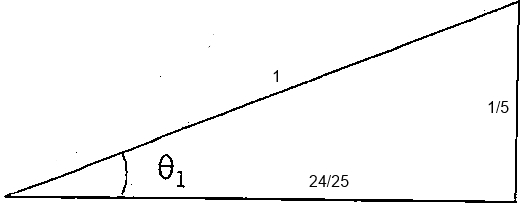
\includegraphics[angle=1, width=0.4\textwidth]{figs/ckmfig1.jpg}
\caption{Cabibbo angle $\theta_1$. Lengths represent decay amplitudes}
\label{cabibbo}
\end{figure}

Only one thousandth of the $4\%$ deviation here is accountable from the 3rd generation but for the moment lets look a bit more into the first two generations.
It shall be shown that these subtle effects arising from the 3rd generation decay amplitudes are where the theory upon CP violation was developed from. From \cref{cabibbo} it is seen that the transition within a generation $u\rightarrow d$ is calculated as $\cos\theta$ and across the generation as $\sin\theta$ which actually corresponds to $u\rightarrow s$. Naively presuming only two generations of matter existed, constructing and amplitude matrix of the corresponding transitions based on this would be appropriate, as will be demonstrated in Eqn.(\ref{mat1}). Note that, for the moment, anti-particles have amplitudes that are the same as their matter counterparts \cite{CKM1}.

\begin{equation}\label{mat1}
\left( \begin{array}{ccc} 
A_{ud} & A_{us} \\
A_{cd} & A_{cs}  \\
\end{array} \right)
 = \left( \begin{array}{ccc}
 \cos\theta_{1} & \sin\theta_{1} \\
 -\sin\theta_{1} & \cos\theta_{1} \end{array} \right)\end{equation}

From \cref{cabibbo} it is calculated that $\theta_1\sim 12^{\circ}$. Experimentally this is measured $\theta_1 = 13.1^{\circ}$ \cite{CKM9}.The impact of this was that the decay rate of many hadronic particles could be calculated, akin to lepton decays, with the additional factor of $\cos\theta_1$or $\sin\theta_1$ in the matrix element. At a quick glance of the Weak Lagrangian,
\begin{equation}\label{mat2}
L_{weak} = i\bar{\psi}\gamma^{\mu}(1-\gamma^{5})\partial^{\mu}\psi -q\sum\bar{\psi}\gamma^{\mu}\sigma_{i}(1-\gamma^{5})\psi A_{\mu i} -\frac{1}{4}F_{\mu \nu}F^{\mu \nu}
\end{equation} 
 the interaction term (the second term in Eqn.(\ref{mat2})) is a key element in the vertexes of the Feynman diagram describing the interactions in \cref{fey1}. An element of this, $\gamma$, signifies axial vector coupling with properties which contribute to CPV \cite{CKM2}.

\begin{figure}[h]
\centering
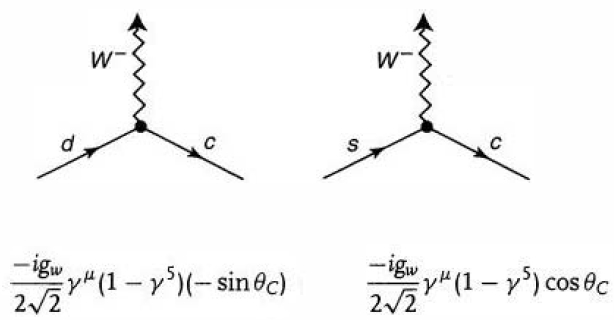
\includegraphics[width=0.5\textwidth]{figs/ckmfig2.jpg}
\caption{Decay amplitudes across generations (Note the Cabbibo angle $\theta_c$ =$\theta_1$). Left $d\rightarrow c$ and right $s\rightarrow c$.}
\label{fey1}
\end{figure}


To progress onto a mechanism for mixing 3 generations of quarks, the first steps must look further into what sets the weak interacting quarks apart from the quarks that are involved in electromagnetic and strong interactions. To begin let us look at an example of the kaon decay into two muons.

\begin{figure}[h]
\centering
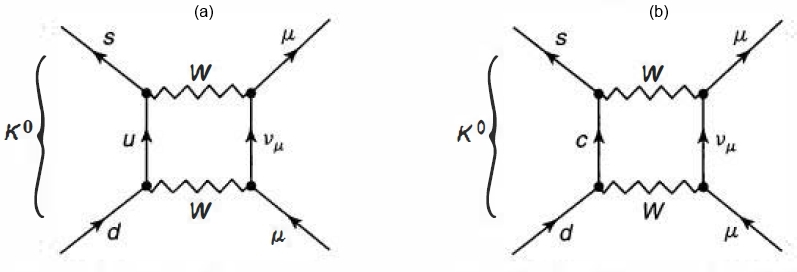
\includegraphics[width=0.5\textwidth]{figs/ckmfig3.jpg}
\caption{Kaon Interfering Feynamn diagrams illustrating GIM mechanism}
\label{fey2}
\end{figure}


So for a decay scheme as the Kaon in \cref{fey2}.a , the virtual up quark is what will be transmitted between the down and strange. This is what would be know as a second order diagram, since the direct decay to a W boson is forbidden. When the amplitudes are found the branching ratio between that and the $K^+\rightarrow\mu\nu$ is calculated to be,
\begin{equation}\label{mat3}
 \frac{K^0\rightarrow\mu\mu}{K^+\rightarrow\mu\nu}=10^{-8}.
\end{equation}
However experimentally this value is found to be too high. What could also be possible is the diagram in \cref{fey2}.b where the virtual quark is now charm. When taking into account these two process we find that in \cref{fey2}.a the amplitude is proportional to $\sin\theta_1 \cos\theta_1$ and in \cref{fey2}.b the amplitude is proportional to $-\sin\theta_1 \cos\theta_1$ on account of $A_{cd}$ in our simple matrix above \cite{CKM5}. 
In 1970, what is called the (Glashow, Iliopoulos and Maiani) GIM mechanism was responsible for a solution \cite{CKM9}. It proposed that ,through the interference with another possible decay process (or diagram) there would be a near cancellation. The remaining value came from the difference in mass between the up and charm quark. Using the experimental Amplitudes this allowed calculations and clear predictions for the mass of the charm quark of about $1.5GeV$. It was successfully discovered in 1974 which then ushered what was known as the November Revolution \cite{CKM2}.
 \\
\\
Cabibbo's theory of mixing together with the GIM mechanism allows for an insightful view of quarks from a different perspective. Instead of one quark that feels the strong, electromagnetic and weak force, there is a sort of mixed phase of quarks involved in weak interactions. So an incognito weak d and s are given by,

\begin{equation}\label{wd}
d' =d\cos\theta_1 +s\sin\theta_1
\end{equation}
 and
\begin{equation}\label{ws}
s'=s\cos\theta_1 -sin\theta_1.
\end{equation}
This can then formulate the matrix,
\begin{equation}\label{mix}
 \left( \begin{array}{c} d' \\  s' \end{array} \right)  = \left( \begin{array}{ccc} cos\theta_1 & sin\theta_1 \\ -sin\theta_1 & cos\theta_1 \end{array}\right) \left( \begin{array}{c} d \\  s \end{array} \right)
\end{equation}
Now the following doublets are found like in leptons using an analogous Cabibbo rotated states,

\begin{equation}\label{mix1}
\left( \begin{array}{c}
 u \\ d'
 \end{array} \right)  = 
\left( \begin{array}{c}
 u \\ d\cos\theta_1 +s\sin\theta_1
 \end{array} \right) \mbox{ and }
 \left( \begin{array}{c}
 c \\ s' \\
 \end{array} \right)  =
 \left( \begin{array}
{c} c \\
 s\cos\theta_1 -d \sin\theta_1 \\
 \end{array}
\right)
\end{equation}
Moving onto a third generation of quarks, the method of finding mixing angles from the Amplitude triangles is repeated.
\begin{figure}[h]
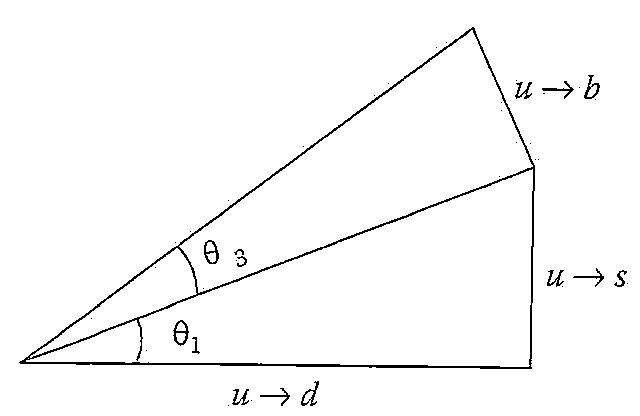
\includegraphics[width=0.3\textwidth]{figs/ckmfig4a.jpg}
\caption{Mixing triangle across 3 generations}
\label{tri3}
\end{figure}

\begin{figure}[h]
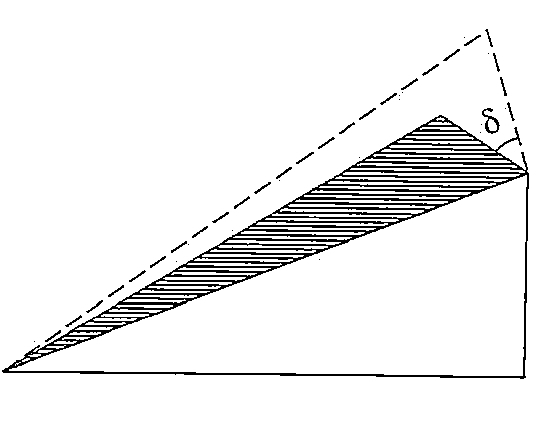
\includegraphics[angle=1.1,width=0.3\textwidth]{figs/ckmfig4b.jpg}
\caption{Complex phase in the 2nd to 3rd generation transitions}
\label{tri4}
\end{figure}

In \cref{tri3} what now is in place is an additional triangle with its base atop the hypotenuse of the 1st to 2nd generation triangle. The transition now facilitates the Amplitude of the up quark transitioning towards the bottom quark path. This gives rise to the angle $\theta_3$ a mixing angle between the 1st and 3rd generation and proceeding with this convention the mixing angle between the 2nd and 3rd is naturally $\theta_2$. The pictorial representation has another hidden feature, \cref{tri4}. The plane the triangle sits in can be thought of as the ‘matter-antimatter mirror’ with the addition freedom of the upper right-angle triangle to swing in and out of the page at an angle $\delta$. It is called the Kobayashi-Maskawa phase, where $\delta=0$ is on the plane of the triangle below. This parameter can set a difference between preferred taste of flavor (quarks and anti-quarks) which will later be shown in Section[IV] and may be the clue to the source of CP violation in nature and perhaps even the structure of the universe itself, but that remains to be seen since in Section[VI] and Section[VII] while still abiding to the conditions that are in place to allow for CP violation , $\delta\neq0$,$\pi$ or $\theta_i\neq0,\frac{\pi}{2}$  \cite{CKM4} .
With a full catalog of mixing between quarks, scaling the prior models to a 3x3 matrix is a task performed in \cite{CKM3} , it incorporates every type of quark mixing in the original formalism. 

\begin{equation}\label{ckm1}
V_{CKM} = \left( \begin{array}{ccc} V_{ud} & V_{us} & V_{ub} \\ V_{cd} & V_{cs} & V_{cb} \\ V_{td} & V_{ts} & V_{tb} \end{array}\right) = \left( \begin{array}{ccc} c_1 & s_1 c_3 & s_1 s_3 \\ -s_1 c_2 & c_1 c_2 c_3 -s_2 s_3 e^{i\delta} & c_1 c_2 s_3 + s_2 c_3 e^{i\delta} \\ -s_1 s_2 & c_1 s_2 c_3 +c_2 s_3 e^{i\delta} & c_1 s_2 s_3 - c_2 c_3 e^{i\delta} \end{array} \right). 
\end{equation}

In order to take advantage of the CKM matrix and illuminate CP violating decays,  two weak amplitudes with complex phase components must exist. An example of such would be the model 4 quark system \cite{CKM4}. Consider two up quarks i and k and two down quarks j and l. Its possible to find that the matrix element is,

\begin{equation}\label{mat4}
M=(V_{ij} V_{kl}) A_1 e^{i \delta_{1}} +(V_{il} V_{kj}) A_2 e^{i\delta_{2}}
\end{equation}

Where $A_1$ and $A_2$ are real value amplitudes and each one represents a unique initial state transitioning to the same final states .The $\delta_1$ and $\delta_2$ are the phases due to higher order processes. The difference between them may be defined as the $\Delta\delta = \delta_1 - \delta_2$ and is known as the CP-even phase. Performing the $\bar{C}\bar{P}$ operation on this matrix element a new one is obtain,

\begin{equation}\label{mat5}
\overline{M}=(V_{ij} V_{kl})^* A_1 e^{i\delta_1} +(V_{il} V_{kj})^* A_2 e^{i\delta_2}
\end{equation}

The two individual amplitudes $A_1$ and $A_2$ in each of the Matrix elements interfere with each other, so to simplify this down for a moment let us absorb the coefficients into $A_1$ and $A_2$ and solve for their decay rates \cite{CKM6}. 
Let,
\begin{equation}\label{amp1}
 \left|A\right|^2 = \left| A_1 +A_2 \right|^2 =\left|  A_1 \right|^2+ \left| A_2 \right|^2 +2\it{R} e\left| A^*_2 A_1 \right| 
\end{equation}

\begin{equation}\label{amp2}
 =\left| A_1 \right|^2 + \left| A_2 \right|^2 +2\left|A_1 A_2 \right| cos(\Delta \phi - \Delta\delta),
\end{equation}
 and
\begin{equation}\label{amp3}
\left| \overline{A}\right|^2 =\left| A_1 \right|^2+ \left| A_2 \right|^2 +2\left| A_1 A_2 \right| cos(\Delta \phi - \Delta\delta),
\end{equation}


The $\phi$ in this case is the CP-even phase. Now defining the CP asymmetry as,

\begin{equation}\label{As1}
\mathbf{A}_{CP} = \frac{\left|A\right|^2-\left|\overline{A}\right|^2}{\left|A\right|^2+\left|\overline{A}\right|^2}
\end{equation}

Apply equation \ref{As1} to \ref{mat4} and \ref{mat5} to find the Asymmetry in our four quark system we solve for the matrix elements. The result is,

\begin{equation}\label{Asm1}
 \mathbf{M}_{CP}= \frac{ 2\it{I}m (V_{ij} V_{kl} V^{*}_{kj }V^{*}_{il} )\sin(\Delta\delta) A_{1} A_{2}}{\left| V_{ij} V_{kl}\right|^2 A^{2}_{1} + \left|V_{kj}V_{il}\right|^2 A^{2}_{2} +2 \it{R} e (V_{ij} V_{kl} V^{*}_{kj} V^{*}_{il} ) \cos(\Delta\delta)A_1 A_2}
\end{equation}\

CP violation in this respect is proportional to $2\it{I}m(V_{ij}V_{kl}V^{*}_{kj}V^{*}_{il})$ which is called $\cal{J}$, the Jacobian. The Jacobian is just the gradient of the scalar valued CKM matrix it also is subject to the same CP violating conditions as what $\delta$ boasted.

So now it may same possible to be stuck with the eternal burden of having a theory with an unknown number of free parameters to test with. To fix this we would like our CKM matrix to be unitary i.e. that itself by it's complex conjugate produces the Identity matrix. A quick glance and a brief frown reveals that the matrix thus far bare no hope unless our off-diagonal elements are relatively small. Hence since CP violation turns out to be very small experimentally and these off diagonal elements are in turn correlated to CPV it has been constructed, in close approximation, a unitary matrix as such. Adopting the Wolfenstein parametrization \cite{CKM10} where we expand on a small parameter $\lambda = 0.22$ to a power series,

\begin{equation}\label{VW1}
V_{W} =\left| \begin{array}{ccc} 1-\frac{\lambda^2}{2} & \lambda & A\lambda^3(\rho-i\nu) \\ -\lambda & 1-\frac{\lambda^2}{2} & A\lambda^2 \\ A\lambda^3(1-\rho-i\nu) &  -A\lambda^2 & 1 \end{array}\right| + {\cal{O}}(\lambda^{4})
\end{equation}
Looking back at the original CKM matrix in \ref{ckm1},
\[\lambda =s_{1}\mbox{  ,    } A=\frac{s_{2}}{s^{2}_{1}}\mbox{  ,    } \rho =\frac{s_{3}}{s_{1}s_{2}}\cos\delta \mbox{ and } \nu = \frac{s_3}{s_1}{s_2}\sin\delta.\]
Comparing this to experimentally measured values CKM matrix elements we have pretty close agreement.
\begin{equation}\label{VEXP1}
V_{exp} = \left( \begin{array}{ccc} 0.9739-0.975 & 0.221-0.227 & 0.0029-0.0045 \\ 0.221-0.227 & 0.9730-0.9744 & 0.039-0.044 \\ 0.0048-0.01 &  0.037-0.043 & 0.9990-0.9992 \end{array}\right) + {\cal{O}}(\lambda^{4})
\end{equation}
\\
As you can see there is a dependence on experimental data but to what extent is it needed. An $n\times n$ complex matrix will have $n^2$ real and complex parameters while unitarity meaning we have $n^2$ constrains. Since we have 6 quarks $(2n)$ which can all have independent phases we have $2n$ fewer parameters. Fixing one phase we then have $n^2 - (2n - 1)$. In the real unitary matrix we have n dimensions and $\frac{n(n-1)}{2}$ free parameters. Thus the total imaginary parameters in the CKM matrix is,
\begin{equation}\label{par1}
n^2 - (2n - 1)-\frac{n(n-1)}{2} = \frac{(n-1)(n-2)}{2}
\end{equation}
 which for n=3 is 1. Hence we have 4 unknown parameters in total, which is why the values of the CKM matrix depend on experimental constraints \cite{CKM7}
\\

As found in \cite{CKM5}, 9 constraints are needed, 6 of which are the sum of complex terms which are zero by orthogonality.  Here are three of these unitary relation equations, 
\begin{equation}\label{par2}
V_{ud}V^{*}_{us}+V_{cd}V^{*}_{cs}+V_{td}V^{*}_{ts}=0,
\end{equation}
\begin{equation}\label{par3}
V_{us}V^{*}_{ub}+V_{cs}V^{*}_{cb}+V_{ts}V^{*}_{tb}=0,
\end{equation}
\begin{equation}\label{par4}
V_{ud}V^{*}_{ub}+V_{cd}V^{*}_{cb}+V_{td}V^{*}_{tb}=0,
\end{equation}

A way to visualize these is as the Unitary triangles in the complex plane and have a surface area of $\frac{\left|\cal{J}\right|}{2}$ \cite{CKM11}. The area is then non-zero for CP violating weak interactions.

\begin{figure}[h]
\centering
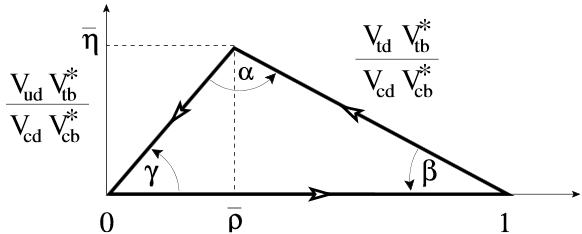
\includegraphics[width=0.5\textwidth]{figs/ckmfig5.jpg}
\caption{Unitary Triangle with angles $\alpha, \beta \mbox{ and } \gamma$}
\label{tri4}
\end{figure}
Now to look a bit closer at the unitary Eqn.(\ref{par4}) to construct the appropriate triangle. In \cref{tri4} a triangle on the basis (x,y) with corners at (0,0), (1,0) and ($\overline{\rho},\overline{\nu}$) is formed, where the reparameterizations are,

\begin{equation}\label{pv1}
\overline{\rho}=\rho\left(1-\frac{\lambda^2}{2}\right) \mbox{ and } \overline{\nu}=\nu\left(1-\frac{\lambda^2}{2}\right)
\end{equation}
The three angles in this diagram $\alpha , \beta \mbox{ and } \gamma$ are defined as,

\begin{equation}\label{ang1}
 \alpha\equiv arg\left(-\frac{V_{tb}V^{*}_{tb}}{V_{ud}V^{*}_{ub}}\right) =\frac{1}{2}\sin^{-1}\left(\frac{2\overline{\nu}(\overline{\nu}^2+\overline{\rho}^2-\overline{\rho})}{(\overline{\rho}^2+\overline{\nu}^2)((1-\overline{\nu})^2+\overline{\nu}^2)}\right) .
\end{equation}

\begin{equation}\label{ang2}
\beta\equiv argl\left(-\frac{V_{cd}V^{*}_{cb}}{V_{td}V^{*}_{tb}}\right) = \frac{1}{2}\sin^{-1}\left(\frac{2\overline{\nu}(1-\overline{\rho})}{(1-\overline{\rho})^2+\overline{\rho}^2}\right).
\end{equation}

\begin{equation}\label{ang3}
\gamma\equiv arg\left(-\frac{V_{ud}V^{*}_{ub}}{V_{cd}V^{*}_{cb}}\right) = \frac{1}{2}\sin^{-1}\left(\frac{2\overline{\rho}\overline{\nu}}{\overline{\rho}^2+\overline{\nu}^2}\right).
\end{equation}

and $\alpha + \beta + \gamma = 180^{\circ}$. Direct measurement of these angles is performed by observations of CP violations in B,D and Kaon meson decays which shall be covered in the following sections \cite{CKM7}.


\section{CPV in Kaon System} 
\vspace{-1.0em}
\begin{center}
\tiny{\textit{Kevin Maguire}}
\end{center}

\subsection{Neutral Kaon Mixing}

As mentioned CPV was first observed in the neutral Kaon system. Direct and indirect CPV have been observed but it is found that the process is entirely dominated by the indirect method. Essential to these mechanisms is the mixing between the neutral Kaon and its anti-particle, corresponding to the states $\ket{K^{0}}$ and $\ket{\bar{K}^{0}}$. These have quark compositions of $d \bar{s}$ and $s \bar{d}$, respectively. 

In interactions involving the strong or EM force, the quantum number strangeness, which tells us the number of strange quarks in a particle, must be conserved. For the weak force it is found that, like parity, this symmetry is not conserved. Due to this many processes forbidden for the strong and EM interactions are allowed through the weak force. This violation is what makes mixing possible. Mixing is the decay of a particle into its anti-particle and can only take place when a particle is its own anti-particle, or if the particles differ by a quantum number which is not conserved by some interaction. This is the case in neutral Kaon mixing, also know as Kaon oscillations. The neutral Kaon and its anti-particle have opposite strangeness but can decay into each other through the strangeness violating weak force. See \cref{KaonMixinFeyn}. 

\begin{figure}[h!]
\begin{center}
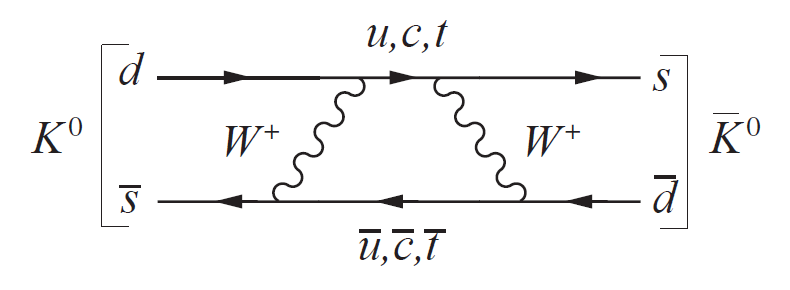
\includegraphics[scale=0.4]{figs/KevFeyn1.png}
\end{center}
\caption{\textit{Feynmann diagram illustrating the process through which neutral Kaons decay into each other}}
\label{KaonMixinFeyn}
\end{figure}

Analogous to the mixing of mass eigenstate quarks to different quark flavours, it is found that the neutral Kaon flavour eigenstates do not correspond to eigenstates of the $\hat{C}\hat{P}$ operator. To show this first operate on the Kaon states with $\hat{C}$. Neglecting phase throughout and assuming no CPV for now, one obtains:

\begin{align*}
\hat{C} \ket{K^{0}(d \bar{s})} = (1)(-1) \ket{\bar{K}^{0}(s \bar{d})} = - \ket{\bar{K}^{0}(s \bar{d})}  \\
\hat{C} \ket{\bar{K}^{0}(s \bar{d})} = (1)(-1) \ket{K^{0}(d \bar{s})} = - \ket{K^{0}(d \bar{s})}  
\end{align*}

\noindent Where we have used the convention that $C (q) = 1$ and ${C} (\bar{q}) = -1$. Also, the action of the $\hat{P}$ operator is given by:
    
\begin{align*}
\hat{P} \ket{K^{0}(d \bar{s})} = {P}(d) {P}(\bar{s})(-1)^{l} \ket{K^{0}(d \bar{s})} = (1)(-1)(-1)^0 \ket{K^{0}(d \bar{s})} = - \ket{K^{0}(d \bar{s})} \\
\hat{P} \ket{\bar{K}^{0}(s \bar{d})} = {P}(s) {P}(\bar{d})(-1)^{l} \ket{\bar{K}^{0}(s \bar{d})} = (1)(-1)(-1)^0 \ket{\bar{K}^{0}(s \bar{d})} = - \ket{\bar{K}^{0}(s \bar{d})} 
\end{align*}

\smallskip

\noindent Where we have used the convention ${P} (fermion) = 1$ and ${P} (anti-fermion) = -1$ as well as $l=0$ because the Kaon is the lowest energy combination of these quarks and itself has a $J^{P}$ of $0^{-}$. Now the eigenstates of $\hat{C}\hat{P}$ can be determined:

\begin{align*}
\hat{C}\hat{P} \ket{K^{0}} = \ket{\bar{K}^{0}} \\
\hat{C}\hat{P} \ket{\bar{K}^{0}} = \ket{K^{0}} 
\end{align*}

\noindent So it is clear that any eigenfunction of the $\hat{C}\hat{P}$ operator will be a linear combination of the two Kaon states:

\begin{align}
\label{FirstKaonLinComb1}
\ket{K^{0}_{1}} = \frac{1}{\sqrt{2}} (\ket{K^{0}} + \ket{\bar{K}^{0}}) \\
\label{FirstKaonLinComb2}
\ket{K^{0}_{2}} = \frac{1}{\sqrt{2}} (\ket{K^{0}} - \ket{\bar{K}^{0}})
\end{align} 

\noindent Where 1 and 2 are the usual labels given to these states. Now the action of $\hat{C}\hat{P}$ on these linear combinations can be determined:

\smallskip

\begin{align*}
\hat{C}\hat{P} \ket{K^{0}_{1}} & = \frac{1}{2} (\hat{C}\hat{P} \ket{K^{0}} + \hat{C}\hat{P} \ket{\bar{K}^{0}}) = \frac{1}{2} (\ket{\bar{K}^{0}} + \ket{K^{0}}) = \ket{K^{0}_{1}} \\
\hat{C}\hat{P} \ket{K^{0}_{2}} & = \frac{1}{2} (\hat{C}\hat{P} \ket{K^{0}} - \hat{C}\hat{P} \ket{\bar{K}^{0}}) =   \frac{1}{2} (\ket{\bar{K}^{0}} - \ket{K^{0}}) = - \ket{K^{0}_{2}} \\
\end{align*} 

In experiment, two Kaon states are observed, a short lived state denoted by $\ket{K^{0}_{S}}$ and a relatively long lived state, $\ket{K^{0}_{L}}$. The lifetimes of these particles are $(8.954 \pm 0.004) \e{-11}$ s and $(5.116 \pm 0.021) \e{-8}$ s, respectively \cite{PDGKaons}. We make the natural assumption that these are the $\hat{C}\hat{P}$ eigenstates just derived and the identifications $\ket{K^{0}_{S}} = \ket{K^{0}_{1}}$ and $\ket{K^{0}_{L}} = \ket{K^{0}_{2}}$, to see what is predicted. If $CP$ is conserved then all the decays of the $\ket{K^{0}_{S}}$ ($CP = 1$) state must be to final products with $CP = 1$, and similarly, the decays of $\ket{K^{0}_{L}}$ ($CP = -1$) must be to final products with $CP = -1$. The observed decays for these states are as follows \cite[pg. 292]{Martin+Shaw}:

\begin{eqnarray*}    
K^{0}_S \rightarrow \pi^0 \pi^0 (B = 0.31),  &   &   K^{0}_{S} \rightarrow \pi^{+} \pi^{-} (B = 0.69)\\ [6pt]
K^{0}_L \rightarrow \pi^0 \pi^0 \pi^0 (B = 0.20),   &   &   K^{0}_{L} \rightarrow \pi^{+}  \pi^{-} \pi^0 (B =0.13)  
\end{eqnarray*}    

\noindent The reason for the difference in lifetimes of these two Kaon states is that the mass of the $K^{0}_L$ is not much bigger than the mass of three pions, thus it is relatively unlikely for it to undergo decay, compared to the $K^{0}_S$ which must only create energy to make two pions. The $CP$ of these final states can now be determined. This is easy for the two pion final states. One finds:

\begin{align}
{P} ({\pi^0 \pi^0})   = & (-1)(-1)(-1)^{l=0} = +1 & \Rightarrow P = 1  \\
{C} ({\pi^0 \pi^0})   = & 1                       & \Rightarrow C = 1  \\
{P} ({\pi^+ \pi^-})   = & (-1)(-1)(-1)^{l=0} = +1 & \Rightarrow P = 1  \\
\label{TwoPionFinalStateCalc}
{C} ({\pi^+ \pi^-})   = & (-1)^{l=0}             & \Rightarrow C = 1 
\end{align}

\noindent Thus ${C}{P} (\pi \pi) = 1$. For the three pion final state the second orbital angular momentum introduced by the third pion must be taken into account. The general formula for such a system is ${P} (ABC) = {P} (A) {P} (B) {P}(C) (-1)^{\mathbf{L}_{AB}} (-1)^{\mathbf{L}_{(AB)C}}$ where $\mathbf{L}_{AB}$ is the orbital angular momentum of the first two pions and $\mathbf{L}_{(AB)C}$ is the orbital angular momentum of the third pion with respect to the mutual centre of mass of the first two pions. The $J^{P}$ of the Kaon is $0^{-}$, thus the overall orbital angular momentum must be zero: $\mathbf{L} = \mathbf{L}_{AB} + \mathbf{L}_{(AB)C} = 0$. As this is angular momentum addition and $\mathbf{L}$ can only take positive values, it is clear that ${L}_{AB} = {L}_{(AB)C}$ so ${L}_{AB} + {L}_{(AB)C} = 2L$, which is an even number: 

\begin{align*}
P(\pi^0 \pi^0 \pi^0)  = & (-1)(-1)(-1)(-1)^{2L = even} = -1 & \Rightarrow P = -1 \\
C(\pi^0 \pi^0 \pi^0)  = & (1)(1)(1) = 1                     & \Rightarrow C = +1 \\
CP(\pi^0 \pi^0 \pi^0) = & -1                                &
\end{align*}

\noindent For the $\ket{\pi^+ \pi^- \pi^0}$ final state the parity is also -1, but the charge conjugation picks up an extra factor of $(-1)^{l}$ as in Eqn.(\ref{TwoPionFinalStateCalc}). So if the centre of mass of pions A and B is taken to be the centre of mass between the $\pi^{+}$ and $\pi^{-}$ one obtains:

\begin{align*}
C(\pi^+ \pi^- \pi^0)  = & C(\pi^{0})(-1)^{{L}_{AB}} = 1     & \Rightarrow C = +1 \\
CP(\pi^0 \pi^0 \pi^0) = & -1                                &
\end{align*}
 
\noindent Where we set ${L}_{AB} = 0$ as higher $L$ values are much less likely \cite{Nakada}. Thus as long as the $K^{0}_{L}$ decay to final states with three pions or other $CP = -1$ states and the $K^{0}_{S}$ only decay to two pion final states or other $CP = 1$ states, then $CP$ is conserved.

This was thought to be the case until in 1964 when Christenson et al discovered the decay mode $K^{0}_{L}(CP = -1) \rightarrow \pi^+ \pi^- (CP = 1)$ with a branching ratio of $(2.3 \pm 0.3) \e{-3}$, thus discovering CPV for the first time \cite{FirstCPV}. The experiment exploits the difference in lifetimes between $K^{0}_{S}$ and $K^{0}_{L}$. A 30GeV proton beam is incident on a metal target which creates a secondary beam of many different particles. The centre of mass energy for such an arrangement is $787~$MeV, which is more than enough energy to produce a neutral Kaon having about a $497~$MeV rest mass. The secondary beam is passed through a magnetic field to remove any charged particles and through a $4~$cm thick block of lead to remove photons. At this point the beam contains both $K^{0}_{S}$ and $K^{0}_{L}$. The detecting apparatus is placed $18~$m away from the metal target, so by the time the beam reaches it, all of the $K^{0}_{S}$ have decayed and only $K^{0}_{L}$ remain. The beam is further collimated and then undergoes collisions in a helium filled bag. Two arms containing a series of detectors are mounted symmetrically around the helium bag, so they both make the same angle with the horizontal. These arms consist of a spark chamber and magnet to determine the momentum and direction of an incident particle. Water Cherenkov and scintillation detectors act as a trigger by only recording events with two oppositely charged particles and a velocity of $0.75~$c to eliminate background, see \cref{Christenson_apparatus}. The aim of the experiment is to measure the angular distribution of produced particles. The results of the experiment are shown in \cref{Christenson_results} where N is the number of counts and $\theta$ is the angle between the net momentum of the detected particles and the initial beam direction. These measurements were taken in various mass ranges, two are shown. If $K^{0}_{L} \rightarrow \pi^+ \pi^-$ is observed, the detected particles will have opposite signs, their invariant mass will match that of $K^{0}_{L}(497)$ and their net momentum will be in the same direction as the incident beam, hence the measured angle will be zero. The results show that a peak occurs at an angle of $0^{\circ}$ in the correct mass range. This is clear evidence of the $CP$ violating decay $K^{0}_{L} \rightarrow \pi^+ \pi^-$.   

\begin{figure}[h!]
\begin{center}
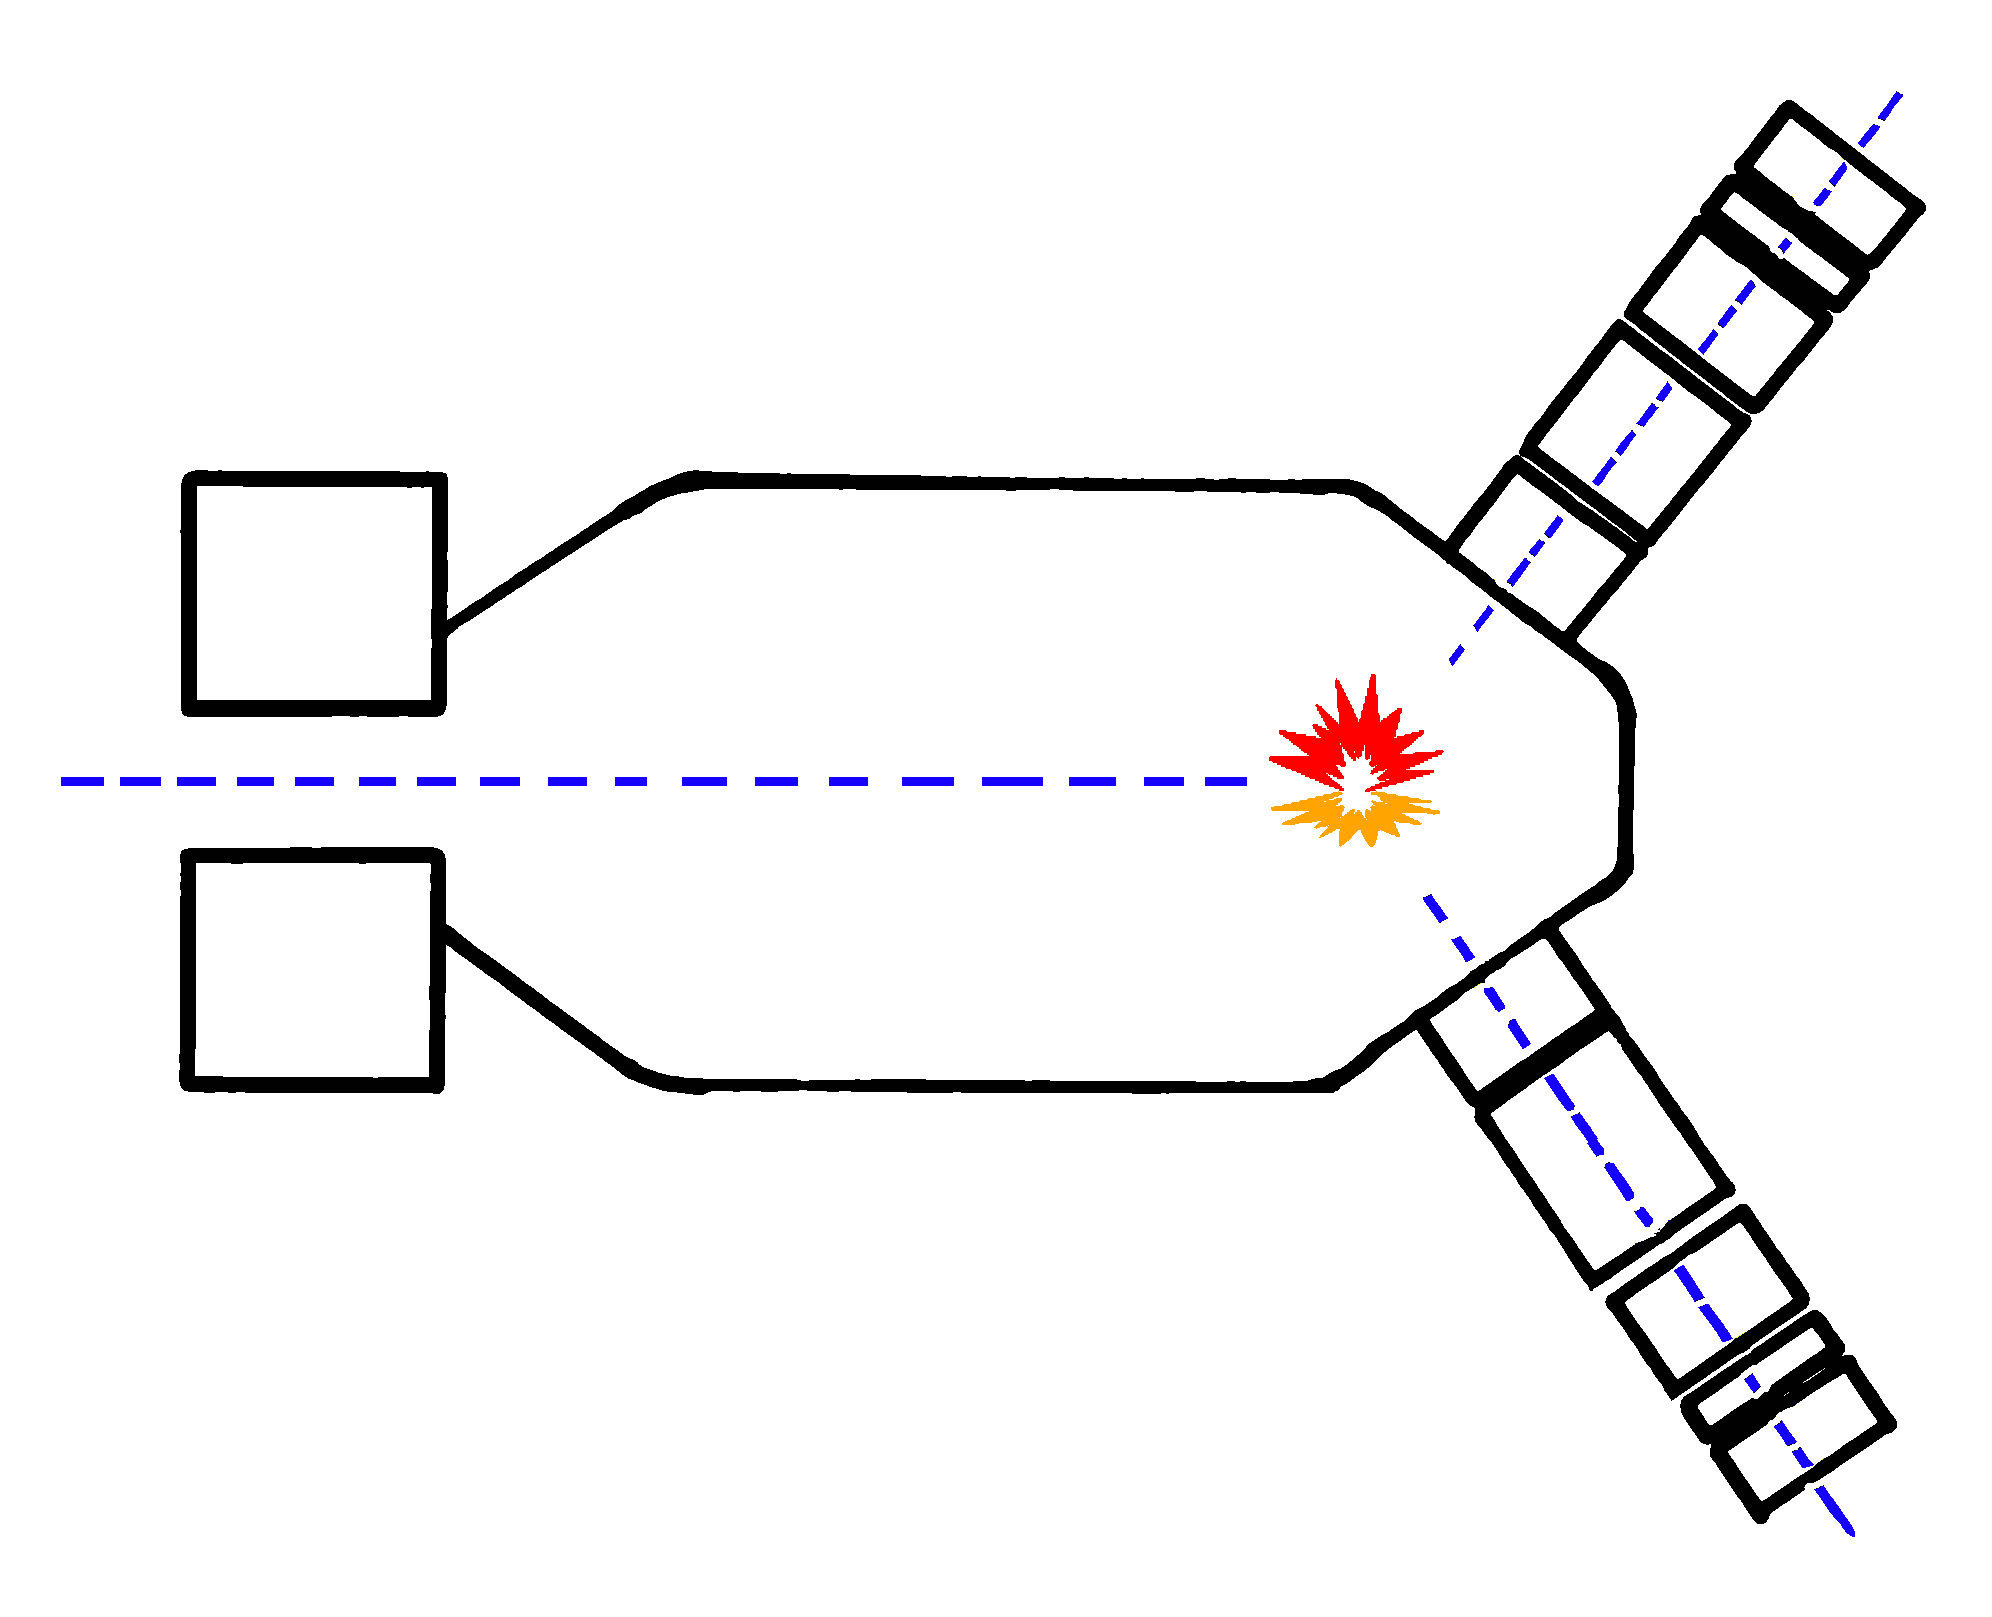
\includegraphics[scale=0.1]{figs/Christenson_apparatus.png}
\end{center}
\caption{\textit{Apparatus used in the Christenson et al experiment \cite{Christenson_apparatus_ref}}}
\label{Christenson_apparatus}
\end{figure}

\begin{figure}[h!]
\begin{center}
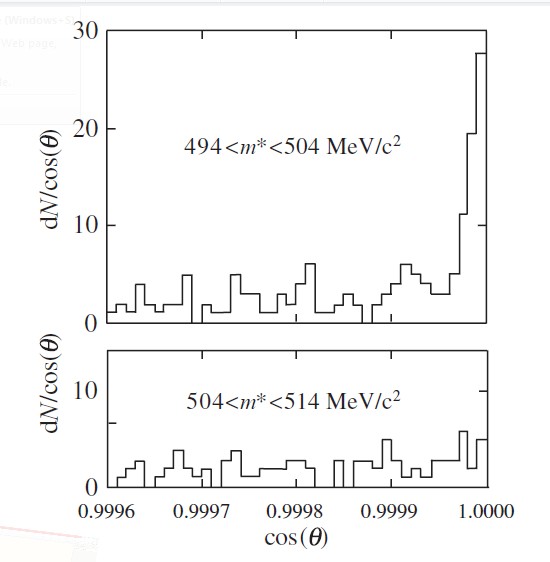
\includegraphics[scale=0.3]{figs/Christenson_results.png}
\end{center}
\caption{\textit{Results of the Christenson et al experiment \cite{FirstCPV}}}
\label{Christenson_results}
\end{figure}

The results of the Christensen et al experiment implies, that the weak eigenstates $\ket{K^{0}_{S}}$ and $\ket{K^{0}_{L}}$ are not aligned with the true $CP$ eigenstates $\ket{K^{0}_{1}}$ and $\ket{K^{0}_{2}}$. As in Eqn.(\ref{FirstKaonLinComb1}) and (\ref{FirstKaonLinComb2}) one can write:

\begin{align}
\label{KaonLincomb11}
\ket{K^{0}_{S}} = a \ket{K^{0}_{1}} + b \ket{K^{0}_{2}} \\
\label{KaonLincomb12}
\ket{K^{0}_{L}} = a \ket{K^{0}_{1}} - b \ket{K^{0}_{2}}
\end{align}

\noindent Where $a$ and $b$ are complex numbers. The degree to which the states are not aligned is determined using the CPV decay amplitudes and corresponding $CP$ conserving amplitudes \cite{Measurements_Direct_CPV_Kaons_KTev}: 

\begin{align*}
\eta_{+-} \vcentcolon= \frac{A(K^{0}_L \rightarrow \pi^+ \pi^-)}{A(K^{0}_S \rightarrow \pi^+ \pi^-)} = \epsilon + \epsilon' \\ 
\eta_{00} \vcentcolon= \frac{A(K^{0}_L \rightarrow \pi^0 \pi^0)}{A(K^{0}_S \rightarrow \pi^0 \pi^0)} = \epsilon - 2\epsilon' 
\end{align*}

\noindent The two complex parameters $\epsilon$ and $\epsilon'$ determine the amount of indirect and direct CPV, respectively. The indirect CPV is due to the $CP$ conserving decay of the $K^{0}_{1}(CP =1)$ component of the $K^{0}_{L}(CP=-1)$ to $CP=1$ final states, this is possible because of Kaon oscillations. The direct CPV is due to the $CP$ violating decay of the $K^{0}_{2}(CP =-1)$ component of the $K^{0}_{L}(CP=-1)$ to $CP=1$ final states, this is possible due to interference between different decay methods with the same final state, as in \cref{HEPP_intro_Perkins}.  

\begin{figure}[h!]
\begin{center}
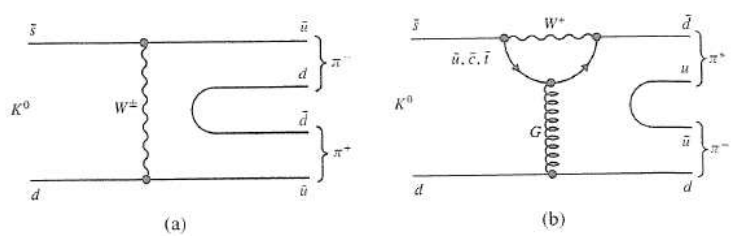
\includegraphics[scale=0.3, angle=-1]{figs/Perkins_Interference_Kaons.png}
\end{center}
\caption{\textit{Two possible decay modes for $K^{0} \rightarrow \pi^+ \pi^-$. (a) Tree diagram for decay by exchanging a W boson (b) Penguin diagram for decay via quark states \cite{HEPP_intro_Perkins}}}
\label{HEPP_intro_Perkins}
\end{figure}

\noindent However it is found that the direct CPV contribution is much smaller in this case. The indirect CPV almost completely dominates as can be seen from the similarity of the experimental values for $|\eta_{+-}|$ and $|\eta_{00}|$ \cite{PDGKaons}:

\begin{align*}
|\eta_{00}| = 0.002220 \pm 0.000011 &  & |\eta_{+-}| = 0.002232 \pm 0.000011 
\end{align*}  

\noindent If these values were significantly different it would suggest the amount of direct CPV would be comparable to the amount of indirect CPV, this of course is not the case. An experimentally determined value which illustrates this is the real part of the ratio of $\epsilon'$ to $\epsilon$ \cite{PDGKaons}:

\begin{equation*}
\mathbb{R} \bigg(\frac{\epsilon'}{\epsilon} \bigg)  = \bigg(1 - \bigg|\frac{\eta_{00}}{\eta{+-}}\bigg|\bigg) / 3 = 0.00166 \pm 0.00023
\end{equation*}

\smallskip

\noindent $|\epsilon|$ can also be determined using:

\begin{equation*} 
|\epsilon| = \big(2 |\eta_{+-}| + |\eta_{00}|\big)/3 = 0.002228 \pm 0.000011
\end{equation*} 

\smallskip

\noindent If the direct CPV contributions are ignored one can write Eqn.(\ref{KaonLincomb11}) and (\ref{KaonLincomb12}) in terms of $\epsilon$:

\begin{align}
\label{KaonLincomb21}
\ket{K^{0}_{L}} = \frac{1}{(1+|\epsilon|^2)^{1/2}} \bigg[ \epsilon \ket{K^{0}_{1}} + \ket{K^{0}_{2}}\bigg] \\
\label{KaonLincomb22}
\ket{K^{0}_{S}} = \frac{1}{(1+|\epsilon|^2)^{1/2}} \bigg[ \ket{K^{0}_{1}} - \epsilon \ket{K^{0}_{2}}\bigg]
\end{align}

\smallskip

\noindent This linear combination shows the non-zero amplitude for weak eigenstate Kaons to oscillate between two different states with definite and opposite $CP$.

\subsection{Semileptonic decays}\label{Kevin:Kaon_semileptonic}

Decays of neutral Kaons to products containing leptons can be used to verify Eqn.(\ref{KaonLincomb21}) and (\ref{KaonLincomb22}) as well as finding the asymmetry in the Kaon oscillation $K^{0} \leftrightarrow \bar{K}^{0}$. First the selection rules that play an important role in these decays must be discussed.

The $\Delta S = \Delta Q$ selection rule is an empirical rule backed up by some theoretical approximations. This rules states that in decays involving strangeness(S) and leptons, the change in the charge(Q) of the hadrons must be the same as the change in strangeness which must have a value of $\pm 1$. As an example consider semileptonic decays of the charged $\Sigma$ baryon. Two semileptonic decays of this baryon are:

\begin{align}
\label{Sigma1}
\Sigma^{-} (dds) \rightarrow n(udd) + e^{-} + \bar{\nu}_{e} \\
\label{Sigma2}
\Sigma^{+} (uus) \rightarrow n(udd) + e^{+} + \nu_{e}
\end{align}  

\noindent The Feynmann diagram for decay (\ref{Sigma1}) can be drawn as in \cref{KevFeyn2}, while decay (\ref{Sigma2}) requires a diagram which must have at least two W bosons. It is clear that the diagram for $\Sigma^{-}$ is quite likely as it contains the Cabbibo favoured quark coupling $V_{ud}$ while any digram with two W bosons is unlikely, as for the $\Sigma^{+}$ decay. For this reason it is highly suppressed and has a branching ratio of $< (5\e{-6})$, which is consistent with it not existing in nature \cite{PDGKaons}. In comparison the decay (\ref{Sigma1}) has a branching ratio of $(1.017 \pm 0.034) \e{-3}$. As there is no selection rule forbidding the second decay, the $\Delta S = \Delta Q$ rule was introduced to identify process like it. The change in strangeness and hadron charge for these decays can be found in \cref{DeltaSQruleTable}.

\begin{figure}[h!]
\begin{center}
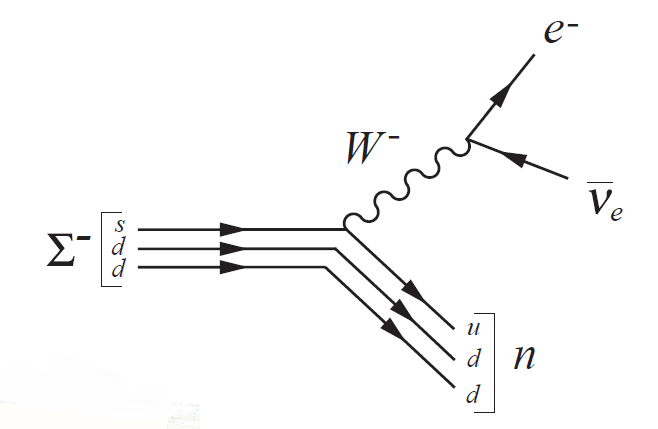
\includegraphics[scale=0.4]{figs/KevFeyn2.png}
\end{center}
\caption{\textit{Feynmann diagram for the $\Delta s = \Delta Q$ allowed decay of the $\Sigma^{-}$ boson to semileptonic final products}}
\label{KevFeyn2}
\end{figure}

\begin{table}[h!]
\caption{\textit{$\Delta S = \Delta Q$ selection rule table for the decays (\ref{Sigma1}) and (\ref{Sigma2})}}
\centering
\setlength{\tabcolsep}{10pt}
\begin{tabular}{c| ccc}
\hline
Shown decay of   & $\Delta S$ & $\Delta Q$ & $\Delta S = \Delta Q$ \\ 
\hline \hline
$\Sigma^{-}$     &      +1    &    +1      & yes                   \\
$\Sigma^{+}$     &      +1    &    -1      & no                   \\
\hline
\end{tabular} 
\label{DeltaSQruleTable}
\end{table}

\smallskip

\noindent Where $\Delta A$ is the difference between the final and initial states of A such that $\Delta A = A_{final} - A_{initial}$. Also remember that the definition of strangeness assigns the strange quark a value of $-1$ and the anti-strange quark a value of $+1$. Thus it is clear that the decay (\ref{Sigma2}) violates the $\Delta S = \Delta Q$ selection rule. Similarly, a decay with $\Delta S = \pm 2$ will contain two W bosons and as a result will be very suppressed. In conclusion, $\Delta S = \Delta Q = \pm 1$ for an allowed process.      

This can now be applied to semileptonic decays of Kaons of the form $K \rightarrow \pi l \nu_{l}$. There are four Kaon decays that have this form:

\begin{align} %maybe put these decays directly into the table below, but may need t refer to them again
\label{Ksemi1}
K^{0} (d \bar{s}) \rightarrow \pi^{-} l^{+} \nu_{l} \\
\label{Ksemi2}
\bar{K}^{0} (s \bar{d}) \rightarrow \pi^{+} l^{-} \bar{\nu}_{l} \\
\label{Ksemi3}
K^{0} (d \bar{s}) \rightarrow \pi^{+} l^{-} \bar{\nu}_{l} \\
\label{Ksemi4}
\bar{K}^{0} (s \bar{d}) \rightarrow \pi^{-} l^{+} \nu_{l} 
\end{align} 

\smallskip

\noindent A similar table as before can now be constructed. See \cref{DeltaSQruleKsemi}, where the number shown refers to the equations above

\begin{table}[h!]
\caption{\textit{$\Delta S = \Delta Q$ selection rule table for the decays (\ref{Ksemi1}) - (\ref{Ksemi4})}}
\centering
\setlength{\tabcolsep}{10pt}
\begin{tabular}{c| ccc}
\hline
Shown decay of  & $\Delta S$ & $\Delta Q$ & $\Delta S = \Delta Q$ \\ 
\hline \hline
(\ref{Ksemi1})  &     -1     &     -1     & yes                   \\
(\ref{Ksemi2})  &     +1     &     +1     & yes                   \\
(\ref{Ksemi3})  &     -1     &     +1     & no                    \\
(\ref{Ksemi4})  &     +1     &     -1     & no                    \\
\hline
\end{tabular} 
\label{DeltaSQruleKsemi}
\end{table}

\noindent Thus it is clear that the only possible semileptonic decays of this form for $K^{0}$ and $\bar{K}^{0}$ are (\ref{Ksemi1}) and (\ref{Ksemi2}). As there is only one way for these processes to occur, there can be no interference between different processes and thus there can be no direct $CP$ violation in the semileptonic decays of Kaons \cite[pg. 10]{DAmbrosio}. So it is clear that the amplitudes of the $\Delta S = \Delta Q$ violating decays are:

\begin{equation*}
A(K^{0} \rightarrow \pi^{+} l^{-} \bar{\nu}_{l}) = A(\bar{K}^{0} \rightarrow \pi^{-} l^{+} \nu_{l}) = 0  
\end{equation*}

It is possible now to write these amplitudes in terms of $K^{0}_{S}$ and $K^{0}_{L}$. Using Eqn.(\ref{FirstKaonLinComb1}),(\ref{FirstKaonLinComb2}),(\ref{KaonLincomb21}) and (\ref{KaonLincomb22}) one finds\cite[pg. 11]{DAmbrosio}:

\begin{align*}
A({K}^{0}_{S} \rightarrow \pi^{+} l^{-} \bar{\nu}_{l}) = - A(K^{0}_{L} \rightarrow \pi^{+} l^{-} \bar{\nu}_{l}) = \frac{1 - \epsilon}{\sqrt{2}} A(\bar{K}^{0} \rightarrow \pi^{+} l^{-} \bar{\nu}_{l}) \\  
A({K}^{0}_{S} \rightarrow \pi^{-} l^{+} \nu_{l}) = A(K^{0}_{L} \rightarrow \pi^{-} l^{+} \nu_{l}) = \frac{1 + \epsilon}{\sqrt{2}} A(K^{0} \rightarrow \pi^{-} l^{+} \nu_{l})   
\end{align*}

\noindent Where terms of order $|\epsilon|^{2}$ have been neglected. The quantities $\delta_{L,S}$ can now be defined, which show the tendency for the oscillations $K^{0} \leftrightarrow \bar{K}^{0}$ to favour the matter particle state. Thus making a very small contribution to the matter anti-matter asymmetry

\begin{equation*}
\delta_{L,S} = \frac{A({K}^{0}_{L,S} \rightarrow \pi^{-} l^{+} \nu_{l}) - A({K}^{0}_{L,S} \rightarrow \pi^{+} l^{-} \bar{\nu}_{l})}{A({K}^{0}_{L,S} \rightarrow \pi^{-} l^{+} \nu_{l}) + A({K}^{0}_{L,S} \rightarrow \pi^{+} l^{-} \bar{\nu}_{l})} \vcentcolon= 2 \mathbb{R}(\epsilon)
\end{equation*}

\noindent The experimental value for this quantity is $\delta_{L} = (3.27 \pm 0.12) \e{-3}$. Which clearly indicates a small tendency to favour the matter particle in oscillations. This can also be illustrated graphically by measuring the relative number(N) of $K^{0}$ and $\bar{K}^{0}$ particles over time in a beam consisting initially of $K^{0}$. See \cref{AsymmetryPicFig}

\begin{figure}[h!]
\begin{center}
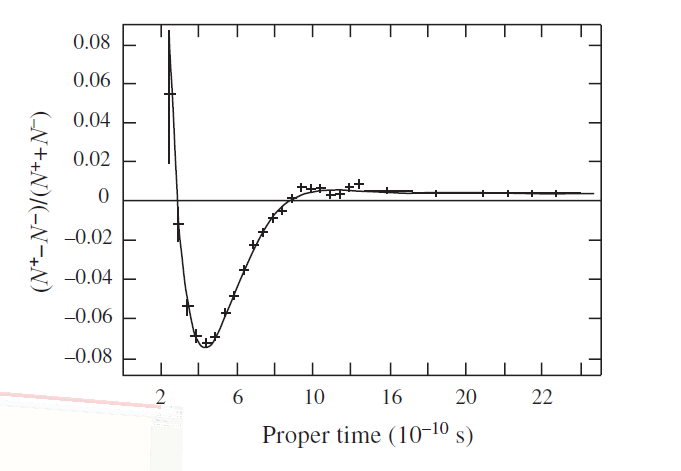
\includegraphics[scale=0.4]{figs/Asymmetry_pic}
\end{center}
\caption{\textit{Measurements of observed Kaon semileptonic decays from a beam initially consisting of $K^{0}$ mesons which shows the oscillation between the states $K^{0}$ and $\bar{K}^{0}$ as well as the small asymmetry, favouring the matter particle \cite{AsymmetryPic}}}
\label{AsymmetryPicFig}
\end{figure}


\subsection{Testing $CPT$ conservation through Strangeness Oscillations}

The $CPT$ theorem links conservation of $CPT$ with Lorentz invariance. Thus to preserve the fundamental Lorentz symmetry physicists desperately hope $CPT$ is conserved. Here is presented some evidence that this is indeed the case. The theorem requires particles and their anti-particles to have the same masses and lifetimes. It has been stated previously that the $K^{0}_{L}$ and $K^{0}_{S}$ particles have very different lifetimes, but thankfully these are not a particle anti-particle pair. From earlier it is clear that $K^{0}$ and $\bar{K}^{0}$ are such a pair. Thus we aim to test $CPT$ conservation by measuring their mass difference.    

By investigating the time evolution of Kaon oscillations it is possible to measure their mass difference. By inverting the linear combinations in Eqn.(\ref{FirstKaonLinComb1}) and (\ref{FirstKaonLinComb2}) and neglecting the very small contribution of $\epsilon$, the flavour eigenstates are described by:

\begin{align*}
\ket{K^{0}(t)} = \frac{1}{\sqrt{2}} (\ket{K^{0}_{S}(t)} + \ket{K^{0}_{L}(t)}) \\
\ket{\bar{K}^{0}(t)}= \frac{1}{\sqrt{2}} (\ket{K^{0}_{S}(t)} - \ket{K^{0}_{L}(t)})
\end{align*} 

\noindent The time evolutions of the states are then written in terms of the mass and the lifetimes of the particles

\begin{align*}
\ket{K^{0}_{S}(t)} = \ket{K^{0}_{S}(0)} e^{-(im_{S}+\Gamma_{s}/2)t} \\
\ket{K^{0}_{L}(t)} = \ket{K^{0}_{L}(0)} e^{-(im_{L}+\Gamma_{L}/2)t} 
\end{align*} 

\noindent Where the exponential factor is as a result of the particle oscillations with time, and the fact that the particle will decay in time. We do the calculation for the $\bar{K}^{0}$ and simply state the result for the $K^{0}$. The probability amplitude(A) for the oscillations and then the probability of decay are determined using the linear combination:

\begin{align}
\ket{\bar{K}^{0}(t)} = \frac{1}{\sqrt{2}} & (\ket{K^{0}_{L}(0)} e^{-(im_{L}+\Gamma_{L}/2)t} - \ket{K^{0}_{S}(0)} e^{-(im_{S}+\Gamma_{s}/2)t}) \\
\bar{A} & = \frac{1}{2} (e^{-(im_{L}+\Gamma_{L}/2)t} - e^{-(im_{S}+\Gamma_{s}/2)t}) \\
\label{StrangenessOscillations1}
P(\bar{K}^{0}) = |\bar{A}|^{2} & = \frac{1}{4} \bigg[ e^{-\Gamma_{S}t} + e^{-\Gamma_{L}t} -2 e^{-(\Gamma_{S} + \Gamma_{L})t/2} \cos(t \Delta m )\bigg] \\
\end{align}

\noindent Where $\Delta m = |m_{S} - m_{L}|$. The extra factor of $1/{\sqrt{2}}$ comes from the initial condition that the experiment is started with a beam of $K^{0}$ particles which is equal parts $K^{0}_{L}$ and $K^{0}_{L}$. Thus $\ket{K^{0}_{L}(t=0)} = \ket{K^{0}_{S}(t=0)} = 1/{\sqrt{2}}$. The corresponding probability for $K^{0}$ is as follows:

\begin{equation}\label{StrangenessOscillations2}
P({K}^{0}) = |{A}|^{2} = \frac{1}{4} \bigg[ e^{-\Gamma_{S}t} + e^{-\Gamma_{L}t} + 2 e^{-(\Gamma_{S} + \Gamma_{L})t/2} \cos(t \Delta m )\bigg] \\
\end{equation}

For this experiment, the initial beam of Kaons is ``flavour tagged''. This is done by producing the $K^{0}$ particles in a strangeness conserving strong decay. The technique of tagging will be discussed further in section [JOHNS SECTION ON B]. The strangeness of the final state particles is then determined by looking for semileptonic decays discussed in section \ref{Kevin:Kaon_semileptonic}. The oscillations in time are made clear by plotting Eqn.(\ref{StrangenessOscillations1}) and (\ref{StrangenessOscillations2}) in \cref{StrangenessOscillationsPic}. The decay rates for $K^{0}_{S}$ and $K^{0}_{L}$ are known so the results of this experiment can be used to determine $\Delta m$ for the weak eigenstate Kaons. This value is $\Delta m = (3.483 \pm 0.006) \e{-12}$.       

\begin{figure}[h!]
\begin{center}
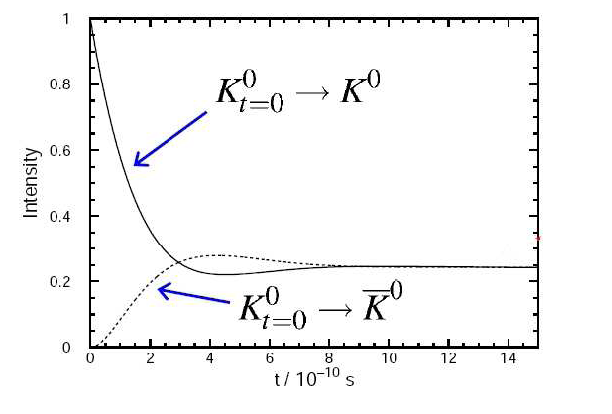
\includegraphics[scale=0.4]{figs/Strangeness_oscillations.png}
\end{center}
\caption{\textit{Theoretical predictions of the strangeness oscillations of a beam initially consisting of $K^{0}$ particles \cite{StrangenessPic}}}
\label{StrangenessOscillationsPic}
\end{figure}

To find ${\Delta m}_{flavour} = |m_{K^{0}} - m_{\bar{K}^{0}}|$ the link between $\Delta m$ above must be determined. The time dependent asymmetry in this system is given by:

\begin{equation*}
A_{CPT} = \frac{P[\bar{K}^{0} \rightarrow \bar{K}^{0}(t)] - P[{K}^{0} \rightarrow {K}^{0}(t)]}{P[\bar{K}^{0} \rightarrow \bar{K}^{0}(t)] + P[{K}^{0} \rightarrow {K}^{0}(t)]} = 4 \mathbb{R}({\delta})
\end{equation*}

\smallskip

\noindent Where $\delta$ is a $CPT$ violation parameter which can be written in terms of its projections parallel and perpendicular to the super weak direction $\phi_{SW} = \tan^{-1} (2 \Delta m / \Delta \Gamma)$ \cite{PDGKaons}:

\begin{align}
\label{CPTstrangeDelta1}
\delta_{\parallel} = \frac{1}{4} \frac{{\Delta \Gamma}_{flavour}}{\sqrt{\Delta m^{2} + \big(\frac{\Delta \Gamma}{2} \big)^{2}}} \\
\label{CPTstrangeDelta2}
\delta_{\perp} = \frac{1}{2} \frac{{\Delta m}_{flavour}}{\sqrt{\Delta m^{2} + \big(\frac{\Delta \Gamma}{2} \big)^{2}}}
\end{align}

Thus it is possible to determine $\mathbb{R}({\delta})$ in this experiment. Using other methods and other experiments $\mathbb{I}m({\delta})$ can be measured. So $\delta_{\parallel}$ and $\delta_{\perp}$ can be determined. Thus as shown in Eqn.(\ref{CPTstrangeDelta2}) $\Delta m_{flavour}$ can be determined. The current best result for this quantity is \cite{PDGKaons}: 

$$\frac{\Delta m_{flavour}}{m_{av}} < 6 \e{-19}$$ 

\noindent which is consistent with zero. Thus this experiment gives some confidence to $CPT$ conservation and the preservation of Lorentz invariance.      
  
  
  
  


%\RequirePackage{fixltx2e}
%\documentclass[floatfix,aps,prd,amsmath,amssymb]{revtex4}
%\usepackage{graphicx}
%\usepackage{caption}
%\usepackage{subcaption}
%\captionsetup{compatibility=false}
%\usepackage[noabbrev,capitalise]{cleveref}
%\usepackage{braket}
%\begin{document}

\section{B mesons and CPV}
\vspace{-1.0em}
\begin{center}
\tiny{\textit{John Ronayne}}
\end{center}

The neutral B-meson is composed of the 1st generation down quark and a 3rd generation bottom quark. While this doesn't contrast the neutral Kaon oscillations to major extent when covering the preliminaries with the benefit of the CKM theory we see that the B-mesons produce a much more dramatic effect.Jumping ahead we define the linear combinations of the B-meson system with egenfunction of $\hat{C}\hat{P}$,
\[\ket{B^{0}_{1}}=\frac{1}{\sqrt{2}}(\ket{B^{0}(d\bar{b})}+\ket{\bar{B}^{0}(\bar{d}b)},\]
\[\ket{B^{0}_{2}}=\frac{1}{\sqrt{2}}(\ket{B^{0}(d\bar{b})}-\ket{\bar{B}^{0}(\bar{d}b)},\]
So including mixing we have the two mass eigenstates,
\[\ket{B_{L}}=p\ket{B^{0}_{1}}+q\ket{{B}^{0}_{2}},\]
\[\ket{B_{H}}=p\ket{B^{0}_{1}}-q\ket{{B}^{0}_{2}},\]
We have adopted the terminology of L for light and H for heavy in relation to the relative masses. We can define mass eigenvalues using the CKM matrix,
\[\frac{q}{p}=\frac{V^{*}_{td}V_{td}}{V_{td}V^{*}_{td}}=e^{-i2\beta}\]
From here we can develop on a few aspects of the B-meson system. To study some direct  \textit{CP} violations we can look at the magnitude  $\left| \frac{q}{p} \right|$. The $\beta$ phase is associated to the mixing and interference and is of interest in experimental measured Indirect  \textit{CP} violation. First the time dependent state must be considered to provide a basis on which the coherent states may be experimentally measured. 


When experimental data is analyzed one B-meson is reconstructed fully (this includes the flavor, B or $\bar{B}$) we call this one $B_{rec}$ with decay time $t_{rec}$ while its sibling is inferred from the decay of the $B_{rec}$ and is called $B_{tag}$ with a $t_{tag}$ decay. The time-depended Asymmetry due to \textit{CPV} in terms of $\Delta{t} = t_{rec}-t_{tag}$ and the number of events N is,
\[\it{A}_{CP}(\Delta t)= \frac{N(B^{0}_{tag},\Delta t)-N(\bar{B}^{0}_{tag},\Delta t)}{N(B^{0}_{tag},\Delta t)+N(\bar{B}^{0}_{tag},\Delta t)},\]



The states $\ket{B^{0}}$ or $\ket{\bar{B}^{0}}$ evolve from t=0 to a pure state of $\ket{B_{phys}^{0}}$ or $\ket{\bar{B}^{0}_{phys}}$ at great t values. 
These states have Decay rate eigenstates as follows,
\[\ket{B(t)}= g_+(t)\ket{B^0}+\left(\frac{q}{p}\right)g_{-}(t)\ket{\bar{B}^0}\]
\[\ket{\bar{B}(t)}= \left(\frac{p}{q}\right)g_-(t)\ket{B^0}+g_{+}(t)\ket{\bar{B}^0}\]
with,
The complete B-meson Amplitude for the decay from a $\Upsilon(4s)$ to the final product of $f_{tag}$ or $f_{rec}$ is,
 \[g_{\pm}(t)=\frac{1}{2}(e^{-i\frac{\Delta m_d \Delta t}{2}}e^{-i\frac{\Delta\Gamma \Delta t}{4}}\pm e^{+i\frac{\Delta m_d \Delta t}{2}}e^{+i\frac{\Delta\Gamma \Delta t}{4}})\]
Which can be shown to equal [ref],
\[g_{+}(t)=e^{-iMt}e^{-\Gamma\frac{t}{2}}\cos(\Delta m_d t/2) \mbox{ and }g_{-}(t)=e^{-iMt}e^{-\Gamma\frac{t}{2}}i\sin(\Delta m_d t/2),\]
when $\Delta\Gamma \approx 0 \mbox{ , }\Delta m_d = 0.502 \pm 0.007 ps^{-1}$, $\Gamma = \frac{1}{\tau_{B^0}}$ and $M=\frac{1}{2}(M_H+M_L)$.

The account for a minus due to the antisymmetric properties of the B-mesons which are produces in a P wave state. To fully expand on this we would require the individual amplitudes for our initialized mesons to decay to either final state. So one meson has the probability to decay to $f_1$ at $t_1$ and the other at $t_2$ to decay to $f_2$. We mentioned $\Delta t$ before but it is of course just $\Delta t = t_1 -t_2$ and $T= t_1 +t_2$.

\[A_{1,2}=\bra{f_{1,2}}\it{H_{Weak}}\ket{B^{0}} \mbox{ and } \bar{A}_{1,2}=\bra{f_{1,2}}\it{H_{Weak}}\ket{\bar{B}^{0}}\]
%\[\it{A} = \braket{f_{tag}|B^{0}_{phys}(t_{tag})} \braket{f_{rec}|\bar{B}^{0}_{phys}(t_{rec})} -\braket{f_{tag}|\bar{B}^{0}_{phys}(t_{tag})} \braket{f_{rec}| B^{0}_{phys}(t_{rec})} \]

A result we can test is ideal. What we can test then is the time-dependent rate of producing a particular decay by the term $\it{F}=\frac{\partial\Gamma}{\partial t}$. 
\[\it{F}(T,\Delta t)=e^{-\Gamma\left|\Delta t\right|}\left| a_{+}g_{+}(\Delta t)+ a_{-}g_{-}(\Delta (t) \right|^{2})\]

the values of $a_+$ and $a_-$ correspond to,

\[ a_{+}=\bar{A}_{tag}A_{rec}-A_{tag}\bar{A}_{rec} \mbox{ and }a_{-}=\left(-\frac{q}{p}\bar{A}_{tag}\bar{A}_{rec}+\frac{p}{q}A_{tag}A_{rec}\right)\]

The use of this shall now be seen but the importance to the understanding of $\it{CP}$ violation is immense. T may be replaced by $\Delta t$ which is a fundamental design capability of detector to measure, this means the physical distance of vertexes of each mason are found. As well as this the coherent states produced mean that the flavor of the particle we detect is fundamentally linked to the paired partner, its tag.

In a time dependent system of coherent states we often define physical properties such a spin or polarization when dealing with light of electrons. Yet the properties ,albeit different follow the same rules. For a system of B mesons the observables we which to examine and the apparent natural asymmetries are found in the eigenstates of either flavor or $\it{CP}$. 

In the case of flavor eigenstates we base our principle of mixing of coherent states. When a B-meson is detected there is a quantum game of chance at play. The $B_{rec}$ is what is seen and we will find it ,through the decay product, to be either a $B^0$ or $\bar{B}^0$ and it partner $B_{tag}$ is found to be the opposite flavor, so  chronologically $\bar{B}^0$ or $B^0$. This is what is know as an unmixed event. The time-dependent rate of decay is thus,
\[F_{unmix}(\Delta t) \propto e^{-\Gamma\left|\Delta t\right|}(1 + cos(\Delta m_d \Delta_t),\]
However there is the other probability. One which we have show to occur is the mixing of of the two B's. Similar to spin flipping in a beam of neutrons or protons we have the flavor being flipped. The $B_{rec}$ having been detected in a $B^0$ or $\bar{B}^0$ state means that the $B_{tag}$ is in the exact same $B^0$ or $\bar{B}^0$ state. Giving a time-dependent rate of decay of,
\[F_{mix}(\Delta t) \propto e^{-\Gamma\left|\Delta t\right|}(1 - cos(\Delta m_d \Delta_t),\]
The oscillations of the B-meson system is directly related to the Mixing asymmetry.
\[A_{mix}(\Delta t) = \frac{F_{unmix}(\Delta t)-F_{mix}(\Delta t)}{F_{unmix}(\Delta t)+F_{mix}(\Delta t)} = cos(\Delta m_d\Delta t) \]

Now we study the eigenstate of $\it{CP}$. Unlike before when the concetration was in the relationship between the two decay products of $B_{rec}$ and $B_{tag}$, we focus purely on our $B_{tag}$ as the CP eigenstate of $B_{rec}$ is assumed. Thus the amplitudes are found from the probable modes of decay. New decay amplitudes are defined on the basis of the final state is accessible due to a $\it{CP}$ operation.
\[A_{f_{CP}}==\bra{f_{CP}}\it{H_{Weak}}\ket{B^{0}} \mbox{ and } \bar{A}_{f_{CP}}=\bra{f_{CP}}\it{H_{Weak}}\ket{\bar{B}^{0}}\]
In scenario (a) the $B_{tag}$ is decaying via a $A_{f_{CP}}$ or $\bar{A}_{f_{CP}}$ while $B_{rec}$ decays as $A_{f_{CP}}$ and in scenario (b) $B_{tag}$ is decaying via a $A_{f_{CP}}$ or $\bar{A}_{f_{CP}}$ while $B_{rec}$ decays as $\bar{A}_{f_{CP}}$. 

Two rates of decay arise on the pretense of the original $B_{tag}$ flavor, these are

\[F(B_{tag}=B^{0},\Delta t) \propto
 e^{-\Gamma |\Delta t|}
\left[1+\frac{1-\left|\frac{q}{p}\frac{\bar{A}_{f_{CP}}}{A_{f_{CP}}}
\right|^{2}}{1+\left|\frac{q}{p}\frac{\bar{A}_{f_{CP}}}{A_{f_{CP}}}\right|^{2}}\cos(\Delta m_{d}\Delta t) - 
\frac{2\it{I}m\frac{q}{p}\frac{\bar{A}_{f_{CP}}}{A_{f_{CP}}}}
{1+\left|\frac{q}{p}\frac{\bar{A}_{f_{CP}}}{A_{f_{CP}}}
\right|^{2}}
\sin(\Delta m_{d} \Delta t)\right]\]
and,
\[F(B_{tag}=B^{0},\Delta t) \propto
 e^{-\Gamma |\Delta t|}
\left[1+\frac{1-\left|\frac{q}{p}\frac{\bar{A}_{f_{CP}}}{A_{f_{CP}}}
\right|^{2}}{1+\left|\frac{q}{p}\frac{\bar{A}_{f_{CP}}}{A_{f_{CP}}}\right|^{2}}\cos(\Delta m_{d}\Delta t) + 
\frac{2\it{I}m\frac{q}{p}\frac{\bar{A}_{f_{CP}}}{A_{f_{CP}}}}
{1+\left|\frac{q}{p}\frac{\bar{A}_{f_{CP}}}{A_{f_{CP}}}
\right|^{2}}
\sin(\Delta m_{d} \Delta t)\right]\]
Again we find the time-dependent asymmetry to be,
\[A_{mix}(\Delta t) = \frac{F_{B_{tag}=B^0}-F_{B_{tag}=\bar{B}^0}}{F_{B_{tag}=B^0}+F_{B_{tag}=\bar{B}^0}} = \frac{1-\left|\frac{q}{p}\frac{\bar{A}_{f_{CP}}}{A_{f_{CP}}}
\right|^{2}}{1+\left|\frac{q}{p}\frac{\bar{A}_{f_{CP}}}{A_{f_{CP}}}\right|^{2}}\cos(\Delta m_{d}\Delta t) - 
\frac{2\it{I}m\frac{q}{p}\frac{\bar{A}_{f_{CP}}}{A_{f_{CP}}}}
{1+\left|\frac{q}{p}\frac{\bar{A}_{f_{CP}}}{A_{f_{CP}}}
\right|^{2}}
\sin(\Delta m_{d} \Delta t)\]

While the shape of the decay rates are in someway unique and a definite property of the asymmetry we wish to observe, the real determination we seek is from the influence of $\Delta t$. This contributes to the amplitude, and the predicted rate which can be observed produced and detected in particle accelerators. As the measurement of such can then be compared back to eqn.[?] to find the $\it{CP}$ angle $\beta$.

%@article{PhysRevD.68.034010,
 % title = {Impact of tag-side interference on time-dependent         \textit{CP}       asymmetry measurements using coherent ${B}^{0}{B}^{0}$ pairs},
%  author = {Long, Owen and Baak, Max and Cahn, Robert N. and Kirkby, David},
%  journal = {Phys. Rev. D},
%  volume = {68},
 % issue = {3},
 % pages = {034010},
 % numpages = {11},
 % year = {2003},
 % month = {Aug},
 % doi = {10.1103/PhysRevD.68.034010},
 % url = {http://link.aps.org/doi/10.1103/PhysRevD.68.034010},
 % publisher = {American Physical Society}
%}

%http://arxiv.org/pdf/hep-ph/9806471v1.pdf
\subsection{BaBar}
While the decay of the Z boson at LEP was initially to study the daughter B-meson particles and their asymmetry a detailed study required a more dedicated experiment and one which B-meson were the sole product. What are called 'B-factories' were designed. BaBar (or $B\overline{B}$ in Stanford and Belle in Japan are experiments which create these B-meson in large quantities (by large we mean 10 per second). We  focus our attention on the BaBar experiment and how it produces and detects the B-mesons. The linear accelerator injects two high energy beams (electrons and positrons) into a circular collider PEP-II. Unlike most colliders the two beams are accelerated to different energies. In particular the electron beam has an energy of 9GeV and the positron beam has an energy of $3.1GeV$. The energy at the center of mass is correspondingly 

\begin{figure}[h]
\centering
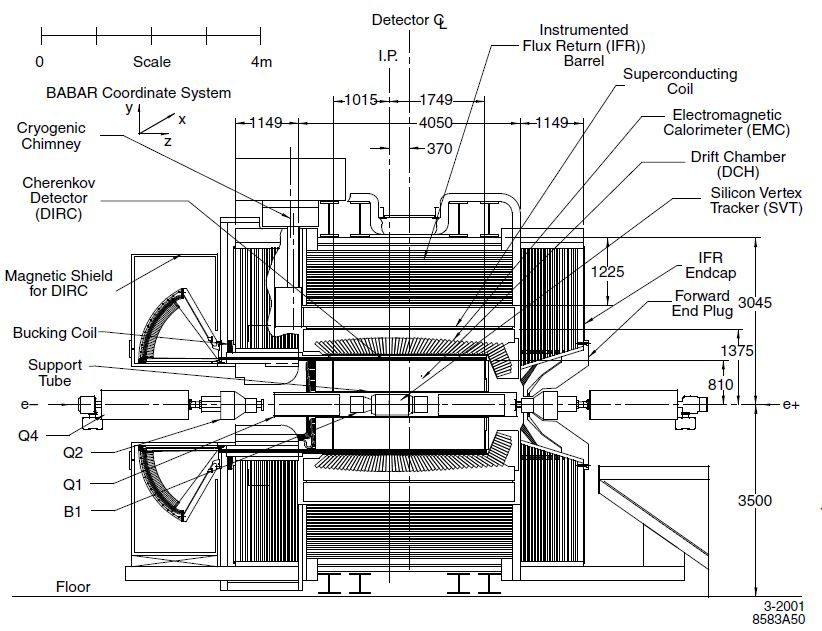
\includegraphics[width=0.75\textwidth]{figs/BBD.jpg}
\caption{The BaBar Detector Schematics}
\label{BBD}
\end{figure}



[working of C.o.M energy ~10.58GeV]

At 10.58GeV it is capable of producing an $\Upsilon(4s)$ which quickly decays to either a $B^+B^-$ or $B^0\overline{B}^0$ pair. Since the Upsilion rest mass is only just enough to create the pair the asymmetric energy beam provides the momentum to separate the pair.
[Fiddlieman Diagram of decay and production]
The uniqueness of this imbalance in momentum gives B-mesons addition momentum upon creation relative to the laboratory centre of mass frame. The benefit is that the distances the B-mesons travel are the measureable and due to time dilation induced by their high velocity the lifetime of the B and $\overline{B}$ mesons can be determined and compared to considerable accuracy. [1]. The calculauble separation that the B’s travel are on average 260um [2]. The Upsilons decays to the $B^0 \overline{B}^0$ pair a quarter of  the total hadronic cross section [citation+decay table]. Thus the luminosity of the beam need to be significantly high to have a reliable amount of data.
The detector itself is the heart of the experiment and where some marvelous engineering and physics has been implemented to preform a detailed study of very specific decays with incredible high fidelity. The $\Upsilon(4s)$ is produced at the interaction point as shown in figure[??] and while the decay products are sweep through the detector via their own momentum or through the 1.5T magnetic field produced by the superconducting coils. 

\begin{figure}[h]
\centering
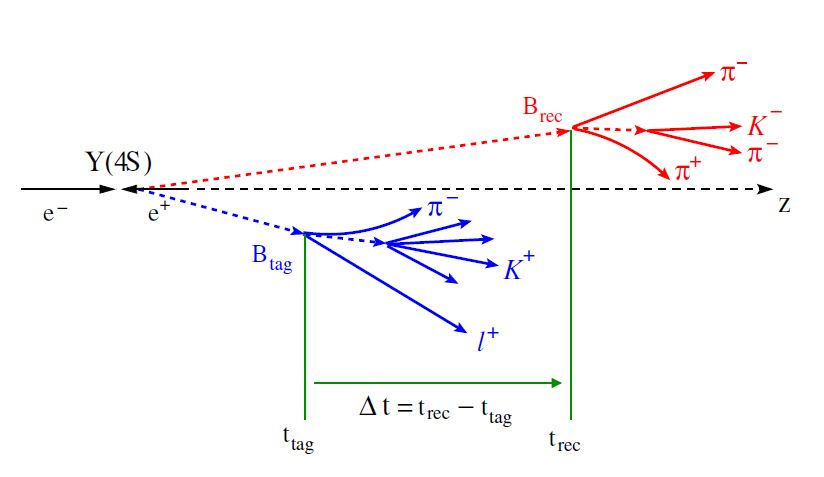
\includegraphics[width=0.75\textwidth]{figs/dt.JPG}
\caption{$\Upsilon (4s)$ decay illustrating the crucial experimental parameter $\Delta t$}
\label{BBD}
\end{figure}


\begin{itemize}
\item The Silicon Vertex Tracker(SVT) consists of five-layers of double sided silicon orientated as interlacing wafers along the inner most part of the detector. Residing only 3.2cm from the center of the 2.7cm radius beam pipe it receives  high fidelity detention of high energy charged particles and low energy e+ e- pairs to an resolution of 10 microns.[a1] The primarily purpose is to contribute to the measurement of the angular and vertex information (the z  and r - $\phi$)of each track which corresponds to the $\Delta z$ resolution where the z-axis is the parallel to the beam. The design had taken into consideration the asymmetric beam energy with the length of each layer increasing relative to the $x-y$ plane and shifted further down the z axis (along the higher energy beam path). [diagram2]. Another design consideration to put in place was the radiation protection. Given the high luminosity of the beam and higher probability of Coulomb scattering inside the pipe the electronic were made to withstand the near $250kRad$ per year [a.1].


%[a1]http://hep.ucsb.edu/people/claudio/Vancouver.pdf
%[a2]http://www.slac.stanford.edu/cgi-wrap/getdoc/slac-pub-11695.pdfm


\item The Drift Chamber(DC) is responsible for measurements of the moment of produced particles as well as information on identifying particles that lose energy inside (the value of $dE/dt$). It extends from the edge of the SVT (22cm) to a radial distance of 80cm . Inside are 7104 small cells connected to tungsten-rhenium sense wires. These wires have a 2kV potential across them and are thick enough to detect the ionized particles while keeping scattering minimal . The chamber contains a gas mixture of 20$\%$ Isobutane and 80$\%$ Helium allowing the atoms to be ionized and detected by the sense wires. [a4]


%http://www.phys.hawaii.edu/superb04/talks/Kelsey.pdf


\item The Detector of Internally Reflected Cerenkov light (DIRC) takes advantage of the Cerenkov radiation. This is a process whereby charged particle traveling at speeds greater than the local speed of light in a medium. Silica rods are placed parallel to the beam pipe surround the outer wall of the Drift chamber. The large index of refraction ($n= 1.474$) means that the speed of light in that medium is only $0.68c$ and a critical angle of about $43^{\circ}$. As charged particle enter the the silica rod and are of sufficient velocity they produce Cerenkov radiation and if it happens to be inside the critical angle it will be internally reflected along the rod to the back of the detector where they enter the "standoff box" containing water and then detected by a ring (correctly speaking a toroidal) of Photomultiplier. Reflecting "light catching cones" capture the light that might otherwise miss the PMT's active surface.  The energy and angle incident angle of each photon is reconstructed during analysis. The primary reason to have a system as such installed is to determine between Kaons and Pions between 0.5 and 4.5$GeV$, this is part of the particle Identification (PID) system. 


%[a3]http://www.slac.stanford.edu/cgi-wrap/getdoc/slac-pub-8080.pdf
\item The EM Calorimeter's (EMC) purpose is to measure the energy and angular resolution between $20MeV$ and $9GeV$. The high energy bar provides detection of the more energetic electrons, muons and photon. Slow moving neutral particles such as the $\pi^0 \mbox{ and the } \eta^0$ will also be detected here.The particles rest mass energy is completely absorbed here due to interactions with the dense material. 6580 Csl(TI) (crystals grown from Csl and doped with 0.1$\%$ Thallium ) trapezoidal crystals are carbon fiber modules .Each Crystal is roughly the dimensions of a standard Rubix cube. Physically it extends a 0.92m to 1.27m and parallel to the pipe 2.3m downstream and 1.5m upstream from the 9GeV beam. At the longer arm length there is an endcap of crystals to facilate the off vertical production of end products, moreover each module is angle towards the central interaction point.

%http://iopscience.iop.org/1742-6596/160/1/012004/pdf/1742-6596_160_1_012004.pdf
\item The Instrument Flux Return (IFR) is separated from the EM Calorimeter by the superconducting coil and the farthest detection instrument from the Interaction point. Here Muons and neutral hadrons (from the light $\pi^0$ to the heavy $K^{0}_{L}$ are detected with the use of the large iron structure needed as the magnetic return yoke. It is segmented into 19 hexagonal layers from 1.8m to 3m from the beam pipe. Between each layer is a single gap resistive plate chamber (RPC) which serve the purpose of detecting ionizing particles such as muon. Muons themselves are identified on the criterion of penetrating ever layer of iron, some slower Muons are identified in the RPCs. 
\end{itemize}
%http://www.slac.stanford.edu/cgi-wrap/getdoc/slac-r-457.pdf
A process of particle Reconstruction and recognition from electronic signatures produced in the detector to the vast system of filtering and discriminating between background process using algorithms and triggering [?] produce reveals the results to compare to our theory.[expand on this]>> The time difference $\Delta t = \frac{\Delta z}{\left< \beta\gamma\right>} c$ is obtained from the measured $\Delta z=z_1 - z_2$ and average boost and average boost $\left<\beta\gamma\right>$. Since the boost is known to good precision, the Dz measurement dominates the $\Delta t$ resolution.
\subsection{Experimental Evidence of $\it{CPV}$ in B-mesons}
Testing B-meson oscillations in the BaBar detector has been accomplished [??] through the di-lepton and semi-leptonic events. Examples of such a decay are 
$B^{0}\rightarrow D^{*-}l^{+}\nu$. By registering charged leptons the flavour of the decayed B-meson can be calculated. Data taken at BaBar are ploted to a likelihood fit. The likelihood fit takes into account the probability of mismatched tags, the resolution of $\Delta t$ and background. In Fig[.a] the unmixed decays are shown where the B-meson pair are of opposite flavor while B-meson pairs that have identical flavors in the mixed state are found in Fig[.b]. Finally the  time dependent asymmetry of the two is found in Fig[.c] clearly exhibiting a cosine wave form as predicted, almost akin to the an inference pattern an undergraduate might observe in laboratories. The frequency of the B-meson oscillations is 80 GHz. Noticeably the amplitude of the Mixed state is significantly lower than unmixed, which is to be expected[detail]. The neutral mixing frequency has been measure to high accuracy at BaBar, the inclusive dilepton sample to be $\Delta m_d = 0.493 \pm 0.012(stat) \pm 0.009(syst) ps^{-1}$.

%@article{PhysRevLett.88.221803,
  %title = {Measurement of the ${\mathit{B}}^{0}-{\overline{\mathit{B}}}^{0}$ Oscillation Frequency with Inclusive Dilepton Events},
 % author = {Aubert, B. et. al},
 %journal = {Phys. Rev. Lett.},
  %volume = {88},
  %issue = {22},
  %pages = {221803},
  %numpages = {7},
  %year = {2002},
  %month = {May},
  %doi = {10.1103/PhysRevLett.88.221803},
  %url = {http://link.aps.org/doi/10.1103/PhysRevLett.88.221803},
  %publisher = {American Physical Society}
%}
 \begin{figure}[h]
\centering
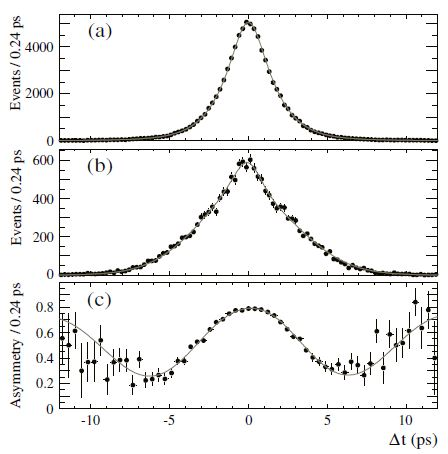
\includegraphics[width=0.5\textwidth]{figs/Flavourosscilatons.JPG}
\caption{(a) Unmixed flavored time dependent decay rate (b) Mixed flavored time dependent decay rate (c) Asymmetry of mixing in flavor eigenstates}
\label{BBD}
\end{figure}

The CP eigenstate decay is on of the most important measurements studied. Much of the theory on CKM matrixes are easily verified by these means. We can approximate our amplitude in eqn[] to something like,
\[\frac{q}{p}\frac{\bar{A}_{f_{CP}}}{A_{f_{CP}}}=\eta_{f_{CP}}e^{2i\beta}, \left|\frac{q}{p}\frac{\bar{A}_{f_{CP}}}{A_{f_{CP}}}\right|=1, \it{I}m\frac{q}{p}\frac{\bar{A}_{f_{CP}}}{A_{f_{CP}}}=-\eta_{f_{CP}}\sin2\beta\]
\[A_{CP}=-\eta_{f_{CP}}\sin2\beta\sin(\Delta m_d \Delta t)\]
To obtain a value for the $\beta $ term we focus on two elements. The $\Delta t$ becomes important and precision measurements of the asymmetry. The Decay of interest here is $B\rightarrow J/\Upsilon K$ [fiddleman diagram here], this is a favorable decay due to the large branching fractions $(\sim 10^{-4})$ and narrow resonance allowing a clean signal above background[ref:recentmes]. In figure[lableit] the asymmetry manifesting due to CP violation is clear visible with the data and likelihood fit corresponding predicted characteristics. The result for $\sin (2\beta) =0.722\pm 0.040_{stat} \pm0.023_{syst}$. Moreover due to ambiguities in the angle $\beta$  and further time depend analysis on the angular decay, $\cos(2\beta)$ is determined an in agreement with the standard model.[ererfe]

 \begin{figure}[h]
\centering
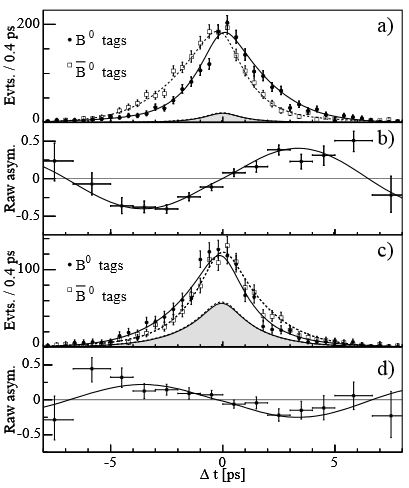
\includegraphics[width=0.36\textwidth]{figs/cpf.JPG}
\caption{(a) Time Distribution in CP odd, $K_{S}$ (b) Raw Asymmetry with likelihood plot (c) Time Distribution in CP even, $K_{L}$  (d)}
\label{BBD}
\end{figure}
%[ererfe]
%@article{PhysRevD.71.032005,
 % title = {Time-integrated and time-dependent angular analyses of $B$\rightarrow${}J/$\psi${}K$\pi${}$: A measurement of $\mathrm{cos}{}2$\beta${}$ with no sign ambiguity from strong phases},
%  author = {Aubert, B.},
%collaboration = {The BABAR Collaboration},
%  journal = {Phys. Rev. D},
%  volume = {71},
%  issue = {3},
%  pages = {032005},
%  numpages = {30},
%  year = {2005},
%  month = {Feb},
%  doi = {10.1103/PhysRevD.71.032005},
%  url = {http://link.aps.org/doi/10.1103/PhysRevD.71.032005},
%  publisher = {American Physical Society}
%}


%@article{Sciolla:2005kz,
%      author         = "Sciolla, Gabriella",
%      title          = "{Recent measurements of sin2b at BABAR}",
%      collaboration  = "BaBar Collaboration",
%      journal        = "Nucl.Phys.Proc.Suppl.",
%      volume         = "156",
%      pages          = "16-20",
%      doi            = "10.1016/j.nuclphysbps.2006.03.054",
%      year           = "2006",
%      eprint         = "hep-ex/0509022",
%      archivePrefix  = "arXiv",
%      primaryClass   = "hep-ex",
%      reportNumber   = "BABAR-PROC-05-030, SLAC-PUB-11485",
%      SLACcitation   = "%%CITATION = HEP-EX/0509022;%%",
%}
%@article{Boos:2004xp,
  %    author         = "Boos, Heike and Mannel, Thomas and Reuter, Jurgen",
     % title          = "{The Gold plated mode revisited: Sin(2 beta) and B0
     %                   ---&gt; J / Psi K(S) in the standard model}",
     % journal        = "Phys.Rev.",
    %  volume         = "D70",
    %  pages          = "036006",
    %  doi            = "10.1103/PhysRevD.70.036006",
     % year           = "2004",
     % eprint         = "hep-ph/0403085",
    %  archivePrefix  = "arXiv",
     % primaryClass   = "hep-ph",
      %reportNumber   = "SI-HEP-2004-04, TTP03-23",
    %  SLACcitation   = "%%CITATION = HEP-PH/0403085;%%",
%}


%\[\left| \frac{\bar{A}_{\bar{f}}} {A_{f}} \right|\neq 1 \]
%\[A_{CP}=\frac{1-\left|\frac{\bar{A}_{\bar{f}}}{A_f}\right|^2}{1+\left|\frac{\bar{A}_{\bar{f}}}{A_f}\right|^2}\neq 2\]
Since we have obtained a $\beta$ term we may now look towards finding a relevant $\gamma$ term to have out unitary triangle near complete. The CKM phase arises from the $V_{ub}$ term in the interferences of $b\rightarrow c \mbox{ and } b \rightarrow u$ transitions, note that the $V_{cb}$ term is phase-less. We construct six possible Feynman diagrams for this process,
\[B^0 \rightarrow D^{*\mp}\pi^{\pm} or B^0 \rightarrow D^{*\mp}\rho^{\pm} \]
The first two are seen in \label{pBGD}. The charged products are clean pointers to a flavor of our $B_{rec}$ meson and we can, as per usual, infer the $B_{tag}$. As per the methods we have used in deriving eqn[??] we follow [ref] to construct the $\it{CP}$ asymmetry term, in terms of j, where j is only a permutation between the various end products of decay.
\[\it{A}^{j}_{\it{CP}}(\Delta t) = \frac{2r^j}{1+\left[r^j\right]^2}\sin(2 \beta +\gamma)cos(\delta^j)\sin(\Delta m_d \Delta t)\]
Since the decay from $\bar{B}^0 \rightarrow D^{*+}\pi^{-}$ is favored via CKM mixing amplitudes over what is called the double-CKM-suppressed decay $B^0 \rightarrow D^{*+}\pi^{-}$ due to two low amplitude mixing terms we see a high sensitivity to the CP angle $\gamma$  \label{kino1} is plot and likelihood fit of the decay distribution. Since measurement of $\gamma$ are still in their infancy the present value is $\gamma = 78^{\circ}\pm12^{\circ}$. We will ignore a discussion on obtaining a value for $\alpha$ since no diirect measurement have been successful made no b transition will produce such a phase. But we can find a value intrinsically by the relations $\sin2\alpha = - \sin(2\beta +2\gamma)$.

%http://cds.cern.ch/record/1106345/files/CERN-THESIS-2008-044.pdf
%MA BAAK thesis/paper
 \begin{figure}[h]
\centering
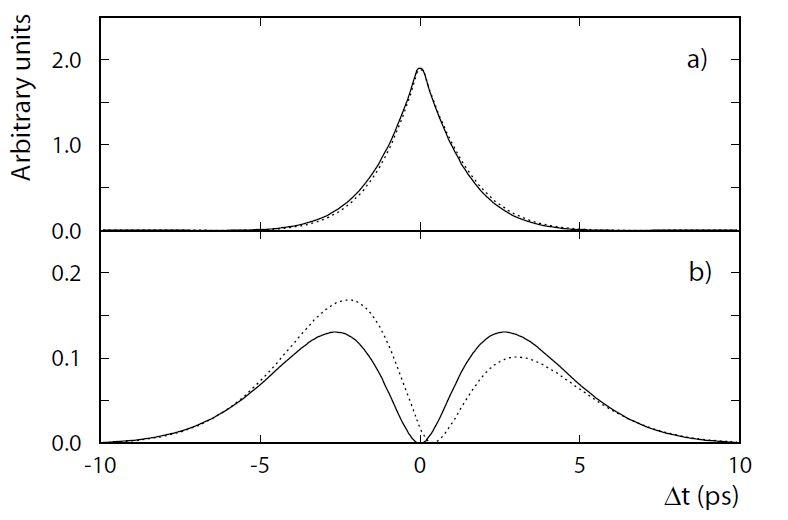
\includegraphics[width=0.6\textwidth]{figs/kino.JPG}
\caption{(a) Time dependent decay for $\bar{B}^0 \rightarrow D^{*-}\pi^{+}$ (b) Time dependent decay for $B^0 \rightarrow D^{*+}\pi^{-}$. If no double-CKM-Suppression were evident the dashed line would be the amplitude.}
\label{kino1}
\end{figure}

 \begin{figure}[h]
\centering
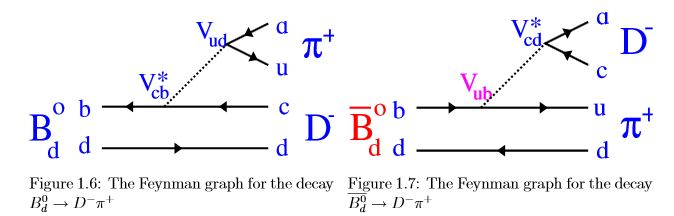
\includegraphics[width=0.8\textwidth]{figs/gam.JPG}
\caption{Convert these puppies to le fiddlemans}
\label{pBGD}
\end{figure}


We have assumed with further explanation the three types of CP violation in this section. Direct being the spontaneous decay via a $\it{CP}$ operation. Indirect being a pure asymmetry in the mixing of B-states and the the combination of the two. Of these there purely indirect has never been observed as the affects are minuscule and dominated in region of high background.


The full range of angle measurement obtainable by B-meson decay are shown in figure [??] .Remarkable the validation of this particular Unitary triangle has stood up to the rigirous measurements made at BaBar and pave a path for the further develepodment of new physics to provide the concrete understanding that lie at the fundamental mechanism of this asymmetry.
 \begin{figure}[h]
\centering
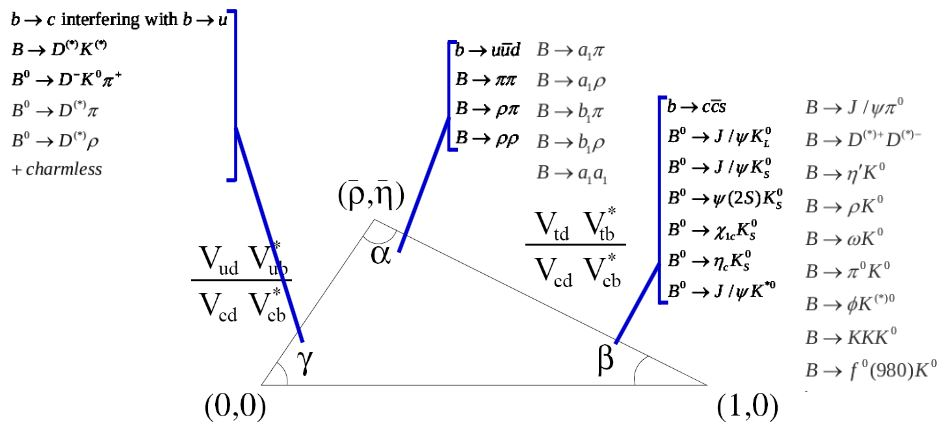
\includegraphics[width=0.8\textwidth]{figs/trig.JPG}
\caption{The B-meson Unitary triangle}
\label{BBD}
\end{figure}

%http://pprc.qmul.ac.uk/~bona/ulpg/cpv/lecture3.pdf


%\end{document}


\section{CPV in D-meson system}
\vspace{-1.0em}
\begin{center}
\tiny{\textit{Kevin Maguire}}
\end{center}

The quark constituents of the $D^{0}(1865)$ and $\bar{D}^{0}(1865)$ mesons are $(c \bar{u})$ and $(u \bar{c})$, respectively. This system is unique as it is the only system which undergoes mixing and contains an up-type quark. As opposed to the $K^{0}$,$B^{0}$ and $B_{S}$, which contain down quarks. This results in different quarks in the mixing box diagrams of these processes, which are illustrated in Fig.(\ref{KevFeyn1.png}) and (\ref{Deon_Mixing_Feyn}). The rates for $D^0$ mixing are expected to be very small as the mixing process shown is suppressed in two ways. If the intermediate quark is a b, then the decay is doubly Cabbibo suppressed[explain? or has it been explained already?], while if the quark is a d or an s then the process is GIM suppressed[Reference John]. Other processes which may not have the same degree of suppression have been proposed, but there are large incertainties in the theoretical calculations of their decay rates \cite{Babar_D0_Review}.    

\begin{figure}[h!]
\begin{center}
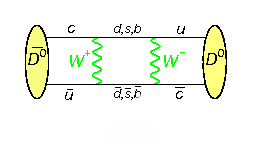
\includegraphics[scale=0.8]{figs/Deon_mixing_feyn.png}
\end{center}
\caption{\textit{Feynmann diagram showing the process by which the two $D^{0}$ states mix. This process is the only known mixing process which contain the d,s,b quarks in this position \cite{Deon_Mixing_Feyn}}}
\label{Deon_Mixing_Feyn}
\end{figure}

The first stage in detecting CPV in any system is to find mixing between a particle and its anti-particle. As in the case of Kaon and B-meson mixing we define the $CP$ eigenstates of the D meson to be linear combinations of flavour eigenstates.

\begin{equation}\label{DeonLinComb}
\ket{D^{0}_{1,2}} = p \ket{D^{0}} \pm q \ket{\bar{D}^{0}}
\end{equation}

\noindent Where for normailzation $|p|^{2}+|q|^{2} = 1$. In the absence of CPV the $\ket{D_{1}}$ state is a $CP$ even state while the $\ket{D_{2}}$ state is a $CP$ odd state. As expected, we will see CPV in mixing if $|p| \neq |q|$. Clear evidence for mixing between these states was announced in 2007 and published in 2008 by the BaBar collaboration, followed shortly by the Belle collaboration \cite{BabarD0mixing}\cite{BelleD0mixing}. Results from both experiments show a small amount of $D^{0}$ mixing with 3.9 $\sigma$ certainty, at a level which is consistent with SM predictions in the order of $|x|,|y| \leq \e{-2}$, see Eqn.(\ref{xyDeonMixing}) \cite{Babar_D0_Review}. However, measured $CP$ violating parameters were consistent with zero, and thus with no CPV.

Two decays and their corresponding anti-particle decays are important for the measuremnt of mixing in the D meson system. The doubly Cabbibo suppressed (DCS) $D^{0} \rightarrow K^{+} \pi^{-}$ known as the wrong sign (WS) decay and $D^{0} \rightarrow K^{-} \pi^{+}$ Cabbibo favoured (CF) decay called the right sign (RS), are used. Two parameters which determine the amount of mixing in a system are defined as:

\begin{align}\label{xyDeonMixing}
x = \frac{\Delta M}{\Gamma} & & y = \frac{\Delta \Gamma}{2 \Gamma}
\end{align}

\noindent where $M= (M_{1}+M_{2})/2$ is average mass,$\Gamma = (\Gamma_{1}+\Gamma_{2})/2$ is average lifetime and $\Delta A \vcentcolon= A_{2} - A_{1}$. An approximation to the time dependence of the WS decay in the absence of CPV is given by \cite{BabarD0mixing}:

\begin{align*}
\frac{T_{WS}(t)}{e^{-\Gamma t}} & \propto R_{D} + \sqrt{R_{D}} y \Gamma t + \frac{{x'}^2 + {y'}^2}{4} (\Gamma t)^{2} \\
                             x' & = x \cos (\delta) + y \sin (\delta)\\
                             y' & = y \cos (\delta) - x \sin (\delta)
\end{align*}

\noindent Where $R_{D}$ is the ratio of the amplitudes of the DCS decay to to CF deacy and $\delta$ is the strong phase difference between the DCS and CF decays. If there is no CPV then we would expect $x' = x$ and $y' = y$. By measuring this time dependence and fitting the results to this formula, it is possible to compare predicted values of x' and y' from various theoretical models and see which best fits the data. Fig.(\ref{BaBar_D0_Mixing_Results.png}) shows the results of the first experiment at BaBar while Fig.(\ref{LHCb_D0_Mixing_Results.png}) shows more recent results from LHCb with a confidence of $5 \sigma$. Flavour tagging of the $D^{0}$ is used in these experiments. The sign of a pion known as the ``slow pion'' from the decay $D^{0*} \rightarrow D^{0} \pi^{+}_{s}$ is compared to the sign of the final product Kaon. Where $D^{0*}$ is a heavier, and thus more energetic version of the $D^{0}$ meson. If the signs are the same, the decay is WS, if they are opposite then the decay is RS. Misidentifying a random pion - not from the $D^{0*}$ decay - as the slow pion causes events which do not contain $D^{0}$ decays to be included in analysis. This creates a background which obstructs the signal data. Other sources of background are misreconstructed $D^{0}$ and combinatorial sources. Misreconstruction is due in part to semi-leptonics decays of the $D^{0}$ or $\bar{D}^{0}$ in which the detector has misidentified a lepton as a pion. Combinartorial background is caused by D mesons being produced not from $D^{0*}$, but from various possible decays of a B-meson. All of these backgrounds are reduced and excluded from the signal decays by making offline cuts to various parameters. These parameters include the the $\chi^{2}$ of the track, vertex and impact parameters of the partilces, the momentum and the mass as well as many others. Mass is plotted in two ways, the reconstructed $D^{0}$ mass distribution $(m_{K \pi})$ and the mass difference between the reconstructed $D^{0*}$ and the $D^{0}$ mass $(\Delta m)$ \cite{Kevin}. Signal events are identifed by a mass peak in the correct place in both $m_{K \pi}$ and $(\Delta m)$, random pion background has a peak in $m_{K \pi}$ but no peak in $(\Delta m)$, and vise versa for misreconstracted particles. Combinatorial background has no peak in either mass distribution. These techniques are of course universal to most particle physics experiemnts. 

\begin{figure}[h!]
\begin{center}
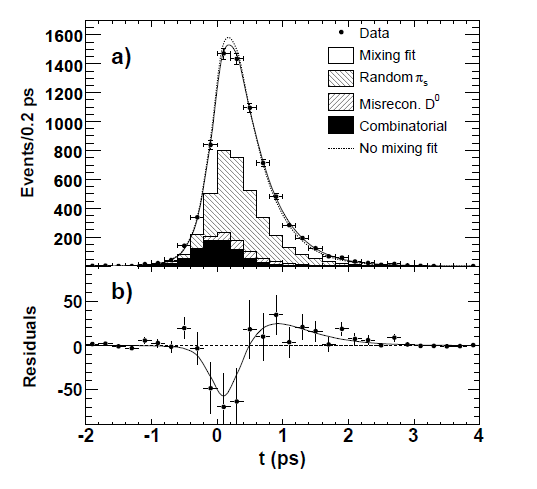
\includegraphics[scale=0.4]{figs/BaBar_D0_Mixing_Results.png}
\end{center}
\caption{\textit{Results from the first $D^{0}$ mixing experiments at BaBar, which plots the time distribution of WS decays. It is clear that the data best fits the mixing hypothesis. Backround contributions from wrongly identified $\pi^{+}_{s}$, misconstructed $D^{0}$ decays and combinatorial contributions from $D^{0}$ production from $B^{0}$ decays are removed}}
\label{BaBar_D0_Mixing_Results.png}
\end{figure}

\begin{figure}[h!]
\begin{center}
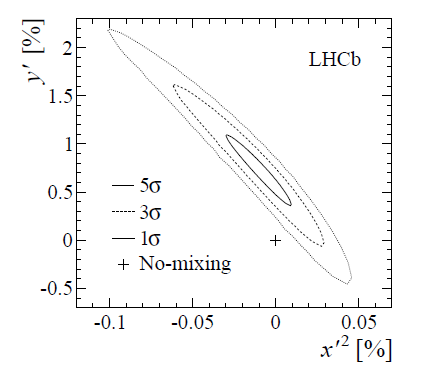
\includegraphics[scale=0.4]{figs/LHCb_D0_Mixing_Results.png}
\end{center}
\caption{\textit{2013 Results from LHCb of $D^{0}$ mixing with a confidence of $5 \sigma$. This is the first conclusive evidence for $D^{0}$ made by one experiemnt. The cross marks the no-mixing values of x' and y'}}
\label{LHCb_D0_Mixing_Results.png}
\end{figure}

CPV in mixing in this system is described by the parameter $A_{m}$ defined by:

\begin{equation*}
A_{m} = \frac{|q/p|^{2} - |p/q|^{2}}{|q/p|^{2} + |p/q|^{2}}
\end{equation*}

\noindent Where p and q are the coeffiiencts in the linear combinations \ref{DeonLinComb}. If this value is found to not be zero then CPV in D meson mixing will be proved. Similarly for direct CPV we define:

\begin{equation*}
A_{d} = \frac{|A_{f}|^{2} - |\bar{A}_{f}|^{2}}{|A_{f}|^{2} + |\bar{A}_{f}|^{2}}
\end{equation*}

\noindent Where $A_{f}$ is the decay amplitude of $D^{0}$ to some final state f, and $\bar{A}_{f}$ is the decay amplitude of $\bar{D}^{0}$ to the state $\bar{f}$. These two parameters can be combined to construct the quantity $\lambda_{f}$ defined by \cite{LHCbAsymmetry}:

\begin{equation*}
\lambda_{f} = \frac{q \bar{A}_{f}}{p A_{f}} = - \eta_{CP} \bigg|\frac{q}{p}\bigg| \bigg|\frac{\bar{A}_{f}}{A_{f}}\bigg| e^{i \phi}
\end{equation*}

\noindent Where $\eta_{CP}$ is the $CP$ eigenvalue of the state f and $\phi$ is the phase between $q/p$ and ${\bar{A}_{f}}{A_{f}}$ and is chosen by convention so that $\ket{D_{1}}$ is an even $CP$ eigenstate. To date there has been no evidence for CPV in the D meson system. Measurements are ongoing at LHCb and if the addition of the 2013 data does not find evidence for CPV then we must wait till the restart of the LHC in 2015. The mush larger luminosity expected after the upgrade will hopefully supply the necessary statistics to conclusively measure a non-zerp value of one of the above parameters. 







\section{Spontaneous Charge Parity Violation} 
\vspace{-1.0em}
\begin{center}
\tiny{\textit{Dudley Grant}}
\end{center}

A major motivation for creating models with new CPV mechanisms is to explain Baryon asymmetry. This is a huge research area, a simple search on arXiv.org reveals over $500$ papers. The most prevalent theories are based around Super-Symmetry (SUSY) and Spontaneous Charge Parity Violation (SCPV). 

Typically these models are created by looking for gauge symmetries which coincide with Lagrangians similar to the Standard Model, but with extra terms that may account for the preference of antimatter to decay into matter.  

SCPV is praised for its ``naturalness" in comparison to regular CPV\cite{SCPV1}. It supposes the possibility to have spontaneous CPV by the vacuum, as opposed to explicit CPV from the CKM matrices. That is, the vacuum is no longer invariant under CP. In a sense this is nice as it may not introduce as many new particles. Indeed, the Minimal SUSY Standard Model is not compatible with SCPV, and in general it is difficult to incorporate SCPV in SUSY models\cite{SCPV1}, but it has been done. For example in SUSY $\mathrm{SO}(10)$ \cite{SCPV2}.

There are two primary goals to this section. First, to elucidate the use of groups in physics, particularly particle physics. Second, to use this knowledge to understand various SCPV  models beyond the insufficient description given in this introduction.

\subsection{Group Theory for Physics}
Some physicists take pride in never having learned group theory and still understanding its applications. This is not an unreasonable point of view, an engineer can launch a rocket without knowing real analysis. 

Undergraduate group theory modules quite commonly focus entirely on groups useful for pure mathematics. This is understandable as it is taught by the math department, but the picture of group theory young physicists may end up with is often quite different to its use in physics.


Part of the reasons groups can be so abstract is that they have very little structure. Even basic physics requires complicated structure. Simply changing coordinates in classical mechanics requires differential geometry, which requires analysis and topology. A \textbf{Group} is a set $G$ with a function $\cdot:G^2\rightarrow G$, having the following properties $\forall g,h,k \in G$
\begin{align*}
\begin{array}{l l l}
(\mathrm{GA}1) & g\cdot h \in G & \text{closure} \\
(\mathrm{GA}2) & \exists e\in G,\phantom{a} e\cdot g = g \cdot e = g \phantom{a}& \text{identity} \\
(\mathrm{GA}3) & \exists g^{-1}\in G, \phantom{a} g^{-1} \cdot g = g \cdot g^{-1} = e & \text{inverse} \\
(\mathrm{GA}4) & (g\cdot h)\cdot k = g\cdot(h \cdot k) & \text{associativity} \\
\end{array}
\end{align*}
Abstract definitions will be avoided in general. To understand this proceed with a useful example. Let $\mathrm{GL}(n,\mathbb{R})$ be the set of all $n\times n$ matrices with real coefficients and non-zero determinant. This forms a group under matrix multiplication.
\begin{itemize}
\item[(GA1)] The product of two $n\times n$ matrices is an $n \times n$ matrix, so it is closed.  
\item[(GA2)] The identity matrix $I$ satisfies $IM=MI=M$.
\item[(GA3)] Non-zero determinant matrices are invertible $M^{-1}M=MM^{-1}=I$.
\item[(GA4)] As real multiplication and addition are associative ($(1+2)+3=1+(2+3)$) Matrix multiplication inherits this property.
\end{itemize}
\textsc{Note:}
\begin{itemize}
\item The set of all real matrices would fail, as zero determinant matrices do not have inverses.
\item Associativity is usually trivial by the definition and not checked.
\end{itemize}
The purpose of this proof was to give some familiar meaning to the abstraction. Detailed proofs shall be avoided in favour of intuition. Note that already  a more powerful structure is present than a group, the field of real numbers, $(\mathbb{R},+,\times)$. This is essentially just two groups glued together, addition and multiplication.

Similarly, every vector space is a group under vector addition. With this it could be said that all of physics uses groups, however a secondary school student does not use differential geometry with Newton's laws. At this stage groups are still useless to the practical physicist.

A \textbf{transformation group} is a more useful idea. Let $X$ be a set, $\mathrm{Transf}(X)$ is the set of all one-to-one functions from $X$ to $X$. This is the set of all ways of rearranging $X$. In the context of a finite group $S=\{1,2,...,n\}$, $\mathrm{Transf}(S)$ is just the set of all permutations. 

If $3$-dimensional space was modelled by $\mathbb{R}^3$ the transformation group would not be useful, it would contain unnatural discontinuous functions that do not relate to intuition about space. What would be useful is:
\begin{center}
The transformations that preserve a property of a space form a group. It is known as the \textbf{invariance group} or the \textbf{symmetry group}.
\end{center}
 This is an extremely general and potent idea. It is also not difficult to prove, so it shall be after the following motivation.
 
Model space again as $\mathbb{R}^3$, transformations should preserve distance. Where Euclidean distance is defined by
\begin{align*}
d(\mathbf{x},\mathbf{y})\vcentcolon = \sqrt{(x_1-y_1)^2+(x_2-y_2)^2+(x_3-y_3)^2}
\end{align*}
 The desired transformation $\mathrm{R}$ has form such that $d(\mathrm{R}\mathbf{x},\mathrm{R}\mathbf{y}) = d(\mathbf{x},\mathbf{y})$. From intuition there are some obvious transformations $\mathrm{R}=I$, the identity matrix, or $\mathrm{R}\mathbf{x} = \mathbf{x}+\mathbf{a}$ a translation in space
\begin{align*}
d(\mathrm{R}\mathbf{x},\mathrm{R}\mathbf{y}) &= d(\mathbf{x}+\mathbf{a},\mathbf{y}+\mathbf{a}) \\
&= \sqrt{\sum_{i=1}^3((x_i+a_i)-(y_i+a_i))^2} \\
&= \sqrt{\sum_{i=1}^3(x_i+a_i-y_i-a_i)^2} \\
&= \sqrt{\sum_{i=1}^3(x_i-y_i)^2} \\
&= d(\mathbf{x},\mathbf{y})
\end{align*}
Now note
\begin{align*}
d(\mathbf{x},\mathbf{y})^2=(\mathbf{x}-\mathbf{y})\cdot(\mathbf{x}-\mathbf{y})
\end{align*}
Where $\cdot$ is the regular dot product. Calling $\Delta\mathbf{x}\vcentcolon =\mathbf{x}-\mathbf{y}$ and using serif font to signify matrix representation
\begin{align*}
\Delta\mathbf{x}\cdot\Delta\mathbf{x} &= \mathsf{\Delta x}^T \mathsf{\Delta x} \\
&= (\mathsf{x}-\mathsf{y})^T(\mathsf{x}-\mathsf{y})
\end{align*}
In other words dot product in an orthonormal basis is a row vector times a column vector. Apply the transformation and assume it preserves distance
\begin{align*}
(\mathrm{R}\mathsf{x}-\mathrm{R}\mathsf{y})^T(\mathrm{R}\mathsf{x}-\mathrm{R}\mathsf{y}) = (\mathsf{x}-\mathsf{y})^T(\mathsf{x}-\mathsf{y})
\end{align*}
The only way this can hold for any $\mathbf{x}$ and $\mathbf{y}$ is if $\mathrm{R}$ is affine, $\mathrm{R}\mathbf{x}=\mathrm{A}\mathbf{x}+\mathbf{a}$ where $\mathrm{A}$ is linear, i.e. a Matrix,
\begin{align*}
(\mathrm{R}\mathsf{x}-\mathrm{R}\mathsf{y})^T(\mathrm{R}\mathsf{x}-\mathrm{R}\mathsf{y}) &= (\mathsf{x}-\mathsf{y})^T(\mathsf{x}-\mathsf{y}) \\
(\mathsf{A}\mathsf{x}+\mathsf{a}-\mathrm{A}\mathsf{y}-\mathsf{a})^T(\mathsf{A}\mathsf{x}+\mathsf{a}-\mathrm{A}\mathsf{y}-\mathsf{a}) &= (\mathsf{x}-\mathsf{y})^T(\mathsf{x}-\mathsf{y})\\
(\mathrm{A}(\mathsf{x}-\mathsf{y}))^T(\mathrm{A}(\mathsf{x}-\mathsf{y})) &= (\mathsf{x}-\mathsf{y})^T(\mathsf{x}-\mathsf{y}) \\
(\mathrm{A}\mathsf{\Delta x})^T(\mathrm{A}\mathsf{\Delta x}) &= \mathsf{\Delta x}^T\mathsf{\Delta x} \\
\mathsf{\Delta x}^T\mathrm{A}^T\mathrm{A}\mathsf{\Delta x} &= \mathsf{\Delta x}^T\mathsf{\Delta x}
\end{align*}
This can only hold if $\mathsf{A}\mathsf{A}^T=I$, so $\mathsf{A}^T = \mathsf{A}^{-1}$. Immediately taking the determinant of both sides gives
\begin{align*}
\det \mathsf{A}\mathsf{A}^T &= \det I \\
\det \mathsf{A} \det \mathsf{A}^T &= 1 \\
\det \mathsf{A} \det \mathsf{A} &= 1 \\
\det \mathsf{A}^2 &= 1 \\
\det \mathsf{A} &\in \{-1,1\}
\end{align*}
This relates to intuition. The determinant of a matrix corresponds to how much it changes a volume. If the determinant of a matrix is $\pm 7$, it will turn a $1$ $m^3$ cube into a $7$ $m^3$ parallelepiped, in order to preserve distance the determinant must have absolute value $1$.

What sort of matrices have determinant $-1$ and $+1$? Consider the examples
\begin{align*}
&\left( \begin{array}{l l l}
1 &0&0 \\
0&-1&0 \\
0&0&1
\end{array} \right) & \left( \begin{array}{l l l}
0&-1&0 \\
1&0&0 \\
0&0&1
\end{array} \right)
\end{align*}
The left matrix represents a reflection in through the xz-plane. The right represents a rotation by $\pi/2$ in the xy-plane. It turns out that all matrices with $\mathsf{A}^T = \mathsf{A}^{-1}$ are either rotations or reflections, together they make the orthogonal group $\mathrm{O}(3)$. A transformation that is an orthogonal matrix plus a translation preserves distance, and the set of all such transformations form a group. Just the usual isometrics of Euclidean space.

Denote the set of rotations, which preserve length and handedness (reflection changes the right hand rule to the left hand rule), as $\mathrm{SO}(3)$, this is also a group.

So far this may seem over simplified but now it is already possible to define groups which preserve much more interesting and relevant properties
\begin{itemize}
\item Galilean Transformations. Preserve Newton's Laws.
\item Unitary Operators. Preserve normalisation in quantum mechanics (QM). Propagators should have this.
\item Lorentz Transformations. Preserve the light cone. Equivalently the Minkowski metric.
\end{itemize}
Intuitively, because these preserve something about a space, they form a group. This can greatly simplify some things, they are always invertible, a composition of two transformations still preserves.

 There are many other aspects of group theory that can be useful here. Consider similar matrices, in the context of groups these are called conjugate elements. In the context of rotations they rotate by the same angle (but not the same direction), in the context of Lorentz Boosts they have the same speed (but not the same direction).
 
 If the reader is interested there is a lot of literature furthering this area, particularly physics-focused is \cite{SCPV3}. In this paper the theory shall not be explained further, aside from the symmetry group theorem proved below. 
\vspace{2mm} \\
\textsc{Theorem:}

{\centering \textit{Consider a set $X$ with a function $f:X\rightarrow Y$, the set of all transformations of $X$ that preserve the function at $x$,\\
$S_f\vcentcolon =\{ T \in \mathrm{Transf}(X) : f(Tx)=f(x), \forall x \in X \}$,\\
$\phantom{a}$ \hspace{48mm} form a group called the \textbf{symmetry group} of $f$.}}
\vspace{2mm} \\

For the example of distance in Euclidean space, $f(Tx)=f(x)$ corresponded to $d(R\mathbf{x},R\mathbf{y}) = d(\mathbf{x},\mathbf{y})$.

\begin{flushleft}\textsc{Proof:} \end{flushleft}

$(\mathrm{GA}1)$ Let $S,T\in S_f$, then
\begin{align*}
f((ST)x=f(S(Tx))= f(Sx) = f(x)
\end{align*}
So $ST$ also preserves $f$, $ST \in S_f$. \\

$(\mathrm{GA}2)$ The identity element of $e$ of $\mathrm{Transf}(X)$ satisfies $f(ex)=f(x)$ by definition of the identity function, so $e \in S_f$.\\

$(\mathrm{GA}3)$  Let $S \in S_f$. Since it is a bijection, an inverse $S^{-1}$ exists. 
\begin{align*}
f(S^{-1}x) = f(SS^{-1}x)= f(ex)= f(x)
\end{align*}
$S$ was introduced as it satisfies $f(Sy)=f(y)$ and pick $y=S^{-1}x$. $S^{-1} \in S_f$.\\

$(\mathrm{GA}4)$ is inherited from $\mathrm{Transf}(X)$. \hfill $\square$\\
\textsc{Note}
\begin{itemize}
\item The proof of the Euclidean transformations is incomplete but trivial to extend. Assume $R$ is affine, show it preserves distance.
\item Strictly speaking symmetry groups should be considered group actions. They act on a set $X$, as matrices act on column vectors.
\end{itemize}
\subsection{Useful Physical Groups}

In the language of symmetry groups, useful physical transformations including the Gauge-symmetry of the Standard Model are investigated.

\begin{flushleft}\textit{example 1.0} The Euclidean Isometries. \end{flushleft}

As was shown in the previous section any combination of rotation, reflection and translation preserve Euclidean distance. This can be extended to n-dimensional Euclidean space $\mathbb{E}^n$, here the group of orthogonal transformations and rotations are denoted respectively as $\mathrm{O}(n)$ and $\mathrm{SO}(n)$.

\begin{flushleft}\textit{example 1.1} Galilean Transformations.\end{flushleft}

Solely preserving distance does not say much about physics. Consider Newton's laws in Cartesian coordinates in an inertial frame with column vector representation
\begin{align*}
m \ddot{\mathsf{x}} = \mathsf{F}
\end{align*}
What sort of transformations $\mathsf{Tx}=\mathsf{Rx}+\mathsf{a}$ preserve this equation? Here $R$ is a function of time, for example transforming to a rotating frame
\begin{align*} 
m \frac{d^2}{dt^2}(\mathsf{Rx+a}) &= \mathsf{RF} 
\\
m \frac{d}{dt}(\dot{\mathsf{R}} \mathsf{x} + \mathsf{R} \dot{\mathsf{x}} )+m\ddot{\mathsf{a}} &= \mathsf{RF} \\
m \frac{d}{dt}(\dot{\mathsf{R}} \mathsf{x} + \mathsf{R} \dot{\mathsf{x}} )+m\ddot{\mathsf{a}}&= \mathsf{RF} \\
m (\ddot{\mathsf{R}} \mathsf{x} + 2\dot{\mathsf{R}} \dot{\mathsf{x}}+\mathsf{R} \ddot{\mathsf{x}} )+m\ddot{\mathsf{a}} &= \mathsf{RF} 
\end{align*}
To have the same form this requires, $\dot{R}=0$ and $\ddot{a}=0$. This is equivalent to saying $R$ is a constant change of basis, such as a rotation, and $\mathsf{a} = \mathsf{v}t + \mathsf{b}$, a translation and a constant velocity. In other words
\begin{align*}
\mathsf{Tx} =  \mathsf{Rx} + \mathsf{a}t+\mathsf{b}
\end{align*}
A Galilean transformation is a symmetry group which preserves Newton's laws. It can be readily extended to also preserve distance and time intervals. \\

The goal is to explain the Quantum Field Theory models, Euclidean distance and Newton's Laws are not applicable. They act as an analogy for the Minkowski metric and QM.

\begin{flushleft}\textit{example 2.0} Lorentz Transformations. \end{flushleft}
Suppose one wishes to preserve the Minkowski Metric, or equivalently, the light-cone. The transformations that do so are called Lorentz transformations, essentially defined by
\begin{align*}
\mathsf{L}^T \mathsf{\eta} \mathsf{L} = \mathsf{\eta}
\end{align*}
Extending the transformations to allow for a translation $P^\mu_\nu x^\nu = L^\mu_\nu x^\nu + a^\mu$, these are called Poincar\'{e} transformations. The essence of Special Relativity is that the laws of physics are invariant under Poincar\'{e} transformation.

\begin{flushleft}\textit{example 2.1} Unitary Transformations. \end{flushleft}
In QM the total probability of a time evolving state must always be $1$, otherwise it is simply not a probabilistic theory. In the context of Hilbert spaces (complex inner product spaces complete under the induced norm), the norm of a state gives its probability, so the norm must be preserved.

Recall in Euclidean space orthogonal transformations preserve the norm of a vector, as it preserves the dot product. The complex result is analogous but in the case of operators extends far more, for example
\begin{align*}
\ket{\Psi(t)}=e^{-it\hat{\mathcal{H}} / \hbar}\ket{\Psi(0)}
\end{align*}
The formal solution to the Sch\"odinger equation, the exponential operator on the right is unitary. In general this has quite complicated form. 

If the Hilbert Space is spanned by a finite set $\{\ket{\psi_1},...,\ket{\psi_n} \}$ it is isometrically isomorphic to the inner product space $\mathbb{C}^n$. To preserve the norm here is similar to $\mathbb{R}^n$

\begin{align*}
|U\mathbf{u}|^2 =(\mathsf{Uu})^{*T}\mathsf{Uu} = \mathsf{u}^{*T}\mathsf{U}^{*T}\mathsf{Uu} = \mathsf{u}^{*T}\mathsf{u} = |\mathbf{u}|^2
\end{align*}
This holds $\forall u \in \mathbb{C}^n$ if and only if  $U^{*T}U=I$. This is similar to orthogonal matrices except there is a complex conjugate. The group of all such matrices is denoted $\mathrm{U}(n)$ and those which have positive determinant form a group $\mathrm{SU}(n)$.

\begin{flushleft}\textit{example 3.0} Classical Electrodynamics. \end{flushleft}
\begin{align*}
\begin{array}{l l l l}
\nabla \cdot \mathbf{E} = \frac{\rho}{\varepsilon} \hspace{6mm}
&\nabla \cdot \mathbf{B} = 0\hspace{6mm}
& \nabla \times \mathbf{E} = -\frac{\partial \mathbf{B}}{\partial t} \hspace{6mm}
&\frac{1}{\mu}\nabla \times \mathbf{B} = \mathbf{j}+\varepsilon\frac{\partial \mathbf{E}}{\partial t}
\end{array}
\end{align*}
As $\nabla \cdot \mathbf{B} = 0$ a theorem shows $\exists \mathbf{A}, \mathbf{B}=\nabla \times \mathbf{A}$ this together with the third equation is
\begin{align*}
\nabla \times \mathbf{E} &= - \partial_t (\nabla \times \mathbf{E}) \\
\nabla \times (\mathbf{E}+\frac{\partial \mathbf{A}}{\partial t}) &=0
\end{align*}
Which in turn gives $\mathbf{E} = -\frac{\partial \mathbf{A}}{\partial t} - \nabla \phi$, where in the time independent case $\phi$ reduced to the electrostatic potential $\phi \vcentcolon = -\int \mathbf{E} \cdot \mathrm{d}\mathbf{x}$


Consider the following transformation
\begin{align*}
\left( \begin{array}{l}
\mathbf{A} \\ \phi
\end{array} \right) \mapsto
\left( \begin{array}{l}
\mathbf{A}+\nabla \lambda \\
\phi - \partial_t \lambda
\end{array} \right)
\end{align*}
These transformed potentials are also valid
\begin{align*}
\nabla \times (\mathbf{A}+\nabla \lambda) = \nabla\times \mathbf{A} + \nabla \times \nabla \cdot \lambda  = \mathbf{B} + 0 \\
-\partial_t(\mathbf{A}+\nabla \lambda)-\nabla (\phi - \partial_t \lambda) = -\partial_t(\mathbf{A})-\nabla \phi = \mathbf{E}
\end{align*}
As these equations are preserved the gauge transformations form a symmetry group. Just as preserving Newton's laws formed a symmetry group. This is an example of a \textbf{gauge transformation}.

More generally a gauge transformation is defined as a \textit{local} transformation that preserves the Lagrangian of a theory. What local means exactly is yet to be defined.

\subsection{Gauge Theory}

The reader may be having a hard time seeing how this relates to particle physics. With the benefit of the language being developed some light may be shed on what the remainder of this section will contain.

Most of the groups discussed have their place in modern particle physics. Lorentz invariance and unitarity of symmetry operators obviously extend from special relativity and QM. That is not all, the gauge-symmetry group of the Standard Model is $\mathrm{SU}(3)\times \mathrm{SU}(2)\times \mathrm{U}(1)$. Many of the popular extensions to the Standard Model are also defined by gauge symmetries such as $\mathrm{SU}(5)$, $\mathrm{SO}(10)$ and $\mathrm{O}(16)$ \cite{SCPV4}.

It is possible to state group conditions used for either (a) deducing that a theory can allow SCPV or (b) creating theories which allow for it\cite{SCPV5}. Explaining how to use this with the mathematics being developed is the primary goal of the section. Although, the hierarchy of knowledge required for theoretical physics is unfortunately large. Despite that the material has attempted to have been presented in a condensed and tangible manner, inevitably some details will be avoided.

In QM overall phase is unimportant, that is $\ket{\psi} \sim \ket{\psi}e^{i\xi}$ where $\xi \in [0,2\pi)$. When making any physical measurement the phase cancels out in the complex inner product. It forms a \textit{global} gauge symmetry. Phase is still important in QM in the form of phase difference. Consider two energy eigenstates with $a,b\in \mathbb{R}$
\begin{align*}
\ket{\psi} &= a\ket{E_1}e^{-iE_1/\hbar} +b \ket{E_2}e^{-iE_2/\hbar} \\
\rightarrow\ket{\psi}e^{iE_1/\hbar} &= a\ket{E_1} +b \ket{E_2}e^{i(E_1-E_2)/\hbar} \\
\braket{\mathbf{x}} &= a^2 \braket{E_1|\mathbf{x}|E_1} +2ab\braket{E_1 |\mathbf{x}|E_2}\cos \theta + b^2 \braket{E_2|\mathbf{x}|E_2}
\end{align*}
So here the phase \textit{difference} $\theta \vcentcolon= (E_1-E_2)/\hbar$ appears explicitly in a measurable quantity. Compare to the phase of the CKM matrix, both phases have physical consequences. It will be shown the case is similar for SCPV. Consider $\mathrm{U}(1)$, a ``matrix" that acts on one-dimensional complex vectors, i.e., complex numbers. In this case then, both the ``matrix" and ``vector" can both be represented as complex numbers 
\begin{align*}
|uz|^2=(uz)^* uz = u^*z^* uz = |z^2||u|^2 = |z|^2
\end{align*}
This holds for all $z$ if and only if $u$ has length 1, so $u = e^{i\xi}$ where $\xi \in [0,2\pi)$. So it can be said that the global phase symmetry of QM can be represented as $\mathrm{U}(1)$. Note that $\mathrm{SU}(1)=\mathrm{U}(1)$ in this case, as the norm of a single complex number must be positive. Likewise as $\mathrm{U}(1)$ represents a rotation in the complex plane it must have the same group structure as $\mathrm{SO}(2)$. In mathematical language the groups are isomorphic, written as $\mathrm{U}(1) \cong \mathrm{SO}(2)$.

Thus it is clearer to say that the global phase invariance group of QM is isomorphic to $\mathrm{U}(1)$. Frequently it is the case that there is a deeper physical meaning behind symmetries. Merely stating a theory is invariant under $\mathrm{U}(1)$ is not sufficient as one must define how $\mathrm{U}(1)$ acts. For example, it can act globally or locally.

Consider Quantum Electrodynamics (QED) the Lagrangian of the theory is invariant under \textbf{local gauge symmetry} of $\mathrm{U}(1)$.
\begin{align*}
\psi(x^0,x^1,x^2,x^3) \mapsto e^{i \xi(x^0,x^1,x^2,x^3)} \psi(x^0,x^1,x^2,x^3)
\end{align*}
Where in Cartesian coordinates $(x^0,x^1,x^2,x^3)=(ct,x,y,z)$. In shorthand
\begin{align*}
\psi(x) \mapsto  \tilde{\psi}(x)=e^{i \xi(x)} \psi(x)
\end{align*}
Where $x\vcentcolon=(ct,x,y,z)$ This inherently insists that phase is irrelevant at any point. It was noted that more structure than merely a group is being used  concerning physical groups. Fields, vector spaces, and vector calculus to name a few. Primarily calculus, a fundamentally geometric structure, appears everywhere in physics. The real scalar function $\xi(x)$ must be differentiable.

This differentiability calls for the structure of a \textbf{Lie group} (acting on a set). A Lie group is simply a group where the group operation and taking inverses are differentiable. For a simple example consider the group of addition on $\mathbb{R}$.
\begin{align*}
&\cdot(x,y) = x+y &\mathrm{inv}(x) = -x
\end{align*}
Both of these functions are differentiable in their arguments so $(\mathbb{R},+)$ forms a Lie Group. Likewise other familiar groups $\mathrm{SU}(n)$, $\mathrm{O}(n)$ and $\mathrm{GL}(n,\mathrm)$ all form Lie groups.

To define calculus on non-Euclidean spaces the structure of differential manifolds is required. The details of which will have to be omitted but some intuitive and useful properties are worth discussing. The dimension of a differential manifold is related to the intuitive understanding of spatial dimension. The surface of a sphere is a two-dimensional space and as expected forms a two-dimensional manifold. This means, for the most part, the sphere can be parametrised by two numbers $(\theta,\phi)$.

$\mathrm{O}(n)$, $\mathrm{U}(n)$ and $\mathrm{SU}(n)$ have manifold dimension $\frac{1}{2}n(n-1)$, $n^2$ and $n^2-1$ respectively. So these objects are no longer purely to be considered as groups but also as abstract smooth geometric spaces.

Returning the example of QED's local gauge symmetry and comparing with the global gauge symmetry of QM
\begin{align*}
\ket{\psi} &\mapsto  \ket{\tilde{\phi}}=e^{i \xi} \ket{\psi(x)} \\
\psi(x) &\mapsto  \tilde{\psi}(x)=e^{i \xi(x)} \psi(x)
\end{align*}
Both symmetries are isomorphic to $\mathrm{U}(1)$ but in very different contexts. In QM it may be regarded simply as a group, but in QED the differentiability effects the Lagrangian non-trivially.

The local gauge symmetry of the strong force is $\mathrm{SU}(3)$ and for the weak force it is $\mathrm{SU}(2)$. Like $\mathrm{U}(1)$ was represented by one parameter which was a function of space-time position $\xi(x)$, $\mathrm{SU}(2)$ and $\mathrm{SU}(3)$ have $2^2-1=3$ and $3^3-1=8$ respectively. Notice peculiarly these these are the amount of force carriers in each theory.

What do these symmetries mean physically? According to \cite{SCPV6}, they are like the the potentials $\mathbf{A}, \phi$ for classical electromagnetism; merely a tool to make the mathematics easier. In the same way as one could use $\mathbf{E}$ and $\mathbf{B}$ without the degeneracy of $\mathbf{A}$ and $\phi$, in principle one could formulate QED completely independent of phase, even without complex numbers.
However the difference between usability would be extreme.


A full treatment of local gauge theory for physics can be found here \cite{SCPV6} and more on Lie groups and differential manifolds related to physics can be found at \cite{SCPV3}. 

The gauge symmetries of the Standard Model are written as the product group $\mathrm{SU}(3)\times \mathrm{SU}(2)\times \mathrm{U}(1)$. A product group is formed in the same way $\mathbb{R}^2$ with vector addition is a product group of $\mathbb{R}\times\mathbb{R}$. This can also be considered a project manifold and indeed it tells us the number of force carriers there are in each theory. Knowing the dimension of the SUSY theory $\mathrm{SU}(5)$ as $5^2-1 = 24$ then tells us the number of force carriers in this theory.

One must call it at a day at some point, actually dealing with Lagrangians is a much more time consuming and worth-while task, but the language developed shall suffice to investigate SCPV models.

\subsection{Group Theoretic Conditions.}
The \textbf{vacuum expectation value} (VEV) of an operator is the expected value of the operator acting on the vacuum state. A vacuum state is analogous to the lowest energy eigenstate of the quantum harmonic oscillator (QHO). For the QHO, the VEV of $\hat{\mathcal{H}}$ is $\hbar \omega /2$. Considering the ladder operators for the QHO analogously to the creation and annihilation operators in QED, this lowest energy state is equivalent to the `no quanta' state. For the remainder of the section the vacuum state for any system shall be denoted  $\ket{0}$.

In the Standard Model vacuum state in general may refer to the vacuum state of different fields. For example in the process of vacuum polarization photons may exist while the electron-positron field is in vacuum state. In order to most generally consider new models abstract scalar fields will be considered. Meaning, $\phi$ need not represent the wave function solely for electromagnetism. It simply represents some interesting field to a new theory.\\

The following is a sketch of a more rigorous development found in \cite{SCPV5}. This paper assumes familiarity with modern Lie Group/Algebra theory and new physics models. Presented below is no substitute, but may be viewed as an intuition-based introduction through the symmetry group language developed.\\

Overall a theory will have a total Lagrangian $\mathcal{L}$ form that depends on every field, just like the total Lagrangian of the Standard Model. Consider first a generalised CP-transformation (GCP), denoted $\hat{G}_{CP}$, on a theory with scalar fields $\phi_i(\mathbf{x},t)$, $i \in \{1,...,n\}$.
\begin{align*}
\phi_i(\mathbf{x},t) \mapsto U_{ij} \phi_j^*(-\mathbf{x},t)
\end{align*}
Where $[U_{ij}]=\vcentcolon\mathsf{U} \in \mathrm{U}(n)$, a symmetric unitary matrix. This is related to regular CP as $\hat{C}\hat{P}\phi(x)=\hat{C}\phi(-x) = c\phi^*(-x)$, where $c\in\mathbb{C}$ and $\phi$ is a scalar field. In column vector form we obtain
\begin{align*}
\left( \begin{array}{c}
\phi_1(\mathbf{x},t) \\
\vdots\\
\phi_n(\mathbf{x},t) \\
\end{array} \right) =\vcentcolon \Phi(\mathbf{x},t) \mapsto \hat{G}_{CP}\Phi(\mathbf{x},t)= \mathsf{U}\Phi^*(-\mathbf{x},t)
\end{align*}
If the total Lagrangian is invariant under this transformation it is GCP invariant.  Now the interest lies in determining the difference between explicit CPV (XCPV) and spontaneous CPV (SCPV). First it is useful to derive conditions where a model is GCP invariant.

So suppose $\mathcal{L}$ is $\hat{G}_{CP}$ invariant. Consider the $\Phi$ as a n-dimensional complex vector. By changing the basis $\Phi \mapsto \mathsf{C}\Phi$, the coordinate transformation for $\mathsf{U}$ is 
\begin{align*}
\mathsf{U} \mapsto \tilde{\mathsf{U}}= \mathsf{CU}\mathsf{C}^\dagger
\end{align*}
Consider $\mathsf{U}$ temporarily as the metric for a complex inner product, by Gram-Schmidt orthonormalisation a change of basis $C$ may be found such that $\tilde{\mathsf{U}}=\mathsf{I}$. In the context of group theory. In this new basis, then, $\hat{G}_{CP}$ reduces to
\begin{align*}
\Phi(\mathbf{x},t) \mapsto \Phi^*(-\mathbf{x},t)
\end{align*}
Merely charge conjugation and reflection of space. Theories are always coordinate invariant, else they are non-physical. Hence the coordinate system $\mathsf{C}\Phi$ may be used. It has thus been shown if a theory is GCP invariant, then coordinates exist where $\mathsf{U}=\mathsf{I}$.\\

\textbf{Explicit CP Violation:}\\
Suppose that $\mathcal{L}$ is invariant under $\hat{G}_{CP}$. As was just shown, there exists a basis where $\mathsf{U}=\mathsf{I}$. Conversely, if for no $\mathsf{U}\in\mathrm{U}(n)$ is $\mathcal{L}$ invariant under $\Phi(\mathbf{x},t) \mapsto \mathsf{U}\Phi^*(-\mathbf{x},t)$ then the theory is explicitly CP violating. Now, this may seem to cover all cases, but, SCPV is not dependent on the GCPV condition. In fact, it is only possible to have SCPV \textit{without} XCPV, as will be explained soon. This must immediately mean that any CPV already observed and predicted by the Standard Model must be explainable in the context of SCPV also.\\

\textbf{Spontaneous CP Violation:}\\
Suppose that $\mathcal{L}$ is invariant under $\hat{G}_{CP}$, this means XCPV cannot happen, however consider the following.

Pick a basis such that $\mathsf{U}=\mathsf{I}$. In this basis suppose that the VEVs (of the GCP operator ) are not all real numbers. Depending on the VEV values it may or may not be possible to change basis again such that all the VEVs are real \textit{and} $\mathsf{U}$ remains equal to $\mathsf{I}$. If it is possible to find such a basis transformation, the model is totally CP-conserving. if it is not, the model has SCPV.

For a somewhat contrived but pedagogic example suppose a model has two scalar fields $\phi_1$ and $\phi_2$. Suppose the Lagrangian they obey is invariant under the following transformation
\begin{align*}
\left( \begin{array}{c}
\phi_1(\mathbf{x},t) \\
\phi_2(\mathbf{x},t)
\end{array} \right) \mapsto \left( \begin{array}{c c}
1 & i \\
-i & 2  
\end{array} \right) \left( \begin{array}{c}
\phi_1^*(-\mathbf{x},t) \\
\phi_2^*(-\mathbf{x},t)
\end{array} \right)
\end{align*}
This has the form of a GCP, as can be verified by checking the matrix is unitary. One can now change basis by
\begin{align*}
\left( \begin{array}{c}
\phi_1(\mathbf{x},t) \\
\phi_2(\mathbf{x},t)
\end{array} \right) \mapsto \left( \begin{array}{c c}
1 & 0 \\
i & 1  
\end{array} \right) \left( \begin{array}{c}
\phi_1(\mathbf{x},t) \\
\phi_2(\mathbf{x},t)
\end{array} \right) = \left(
\begin{array}{c}
\phi_1(\mathbf{x},t) \\
\phi_2(\mathbf(x),t) + i \phi_1(\mathbf{x},t)
\end{array} \right)
\end{align*}
This gives the new $\mathsf{U}$ by
\begin{align*}
\left( \begin{array}{c c}
1 & i \\
-i & 2  
\end{array} \right) \mapsto \left( \begin{array}{c c}
1 & 0 \\
i & 1  
\end{array} \right)\left( \begin{array}{c c}
1 & i \\
-i & 2  
\end{array} \right)\left( \begin{array}{c c}
1 & 0 \\
i & 1  
\end{array} \right)^\dagger 
= \left( \begin{array}{c c}
1 & 0 \\
0 & 1  
\end{array} \right)
\end{align*}
So by changing the basis of the fields there is a simpler representation of GCP, it may make the overall Lagrangian more complicated, but one may simply solve that in the first coordinates for the vacuum state, then write that in the GCP preferred coordinates after.

Assume that $\mathcal{L}$ is invariant under $\hat{G}_{CP}$, that is: The Lagrangian does \textit{not} have XCPV, unlike the Standard Model. Whether SCPV is present or not depends on the VEVs of the $\hat{G}_{CP}$ operator. To obtain these one must explicitly solve $\mathcal{L}$ and find the vacuum state, doing this abstractly one may simply choose example VEVs.\\

\begin{flushleft}\textit{case 1} No SCPV, no XCPV. \end{flushleft} 
Suppose, using the coordinate system obtained where $\mathsf{U}=\mathsf{I}$, that
\begin{align*}
\braket{0|\hat{G}_{CP}|0} = \left( \begin{array}{c} \hbar \omega_1 \\ \hbar \omega_2 \end{array}\right)
\end{align*}
In this case, there is no SCPV. A coordinate basis has been founded with real VEVs and $\mathsf{U} = \mathsf{I}$.

\begin{flushleft}\textit{case 2} SCPV. \end{flushleft} 
Suppose, using the coordinate system obtained where $\mathsf{U}=\mathsf{I}$, that
\begin{align*}
\braket{0|\hat{G}_{CP}|0} = \left( \begin{array}{c} i\hbar \omega_1 \\ \hbar \omega_2 \end{array}\right)
\end{align*}
Here it is impossible to remove the complex number and keep $\mathsf{U}$ as the identity matrix. So there is SCPV. So what is SCPV exactly beyond the mathematical formulation? It means the vacuum is not invariant under CP, but it is not the same CP one is used to as in the Standard Model, as for SCPV to exist XCPV must not. Returning the to earlier discussion about phase invariance in QM, for SCPV to occur one  needs a \textit{physical} phase to occur in the VEVs (for example $i=e^{i\frac{\pi}{2}}$ in the previous example). Just as the physical phase difference occurs when measuring, say, the expected value of position. So these phases do give rise to real physical meaning. Described this way, the phase of the CKM matrix is an easy analogy to understand.

\begin{center}
In quantum physics one must pay attention to which phases have physical consequence. \\Such as: (1) phase-difference between eigenstates in a quantum mechanical state, (2) the\\ phase of the CKM matrix and (3) the relative phases of VEVs in SCP violating theories.
\end{center}


Through the language of symmetry groups the results just obtained are powerful tools for assessing the behaviour of CP in various theories. These initial results are summarised below.
\begin{itemize}
\item[(A)] Invariance of $\mathcal{L}$ under $\hat{G}_{CP}$.
\item[(B)] Having coordinates in which: (i) $\hat{G}_{CP}$ reduces to spatial reflection and conjugation and (ii) the VEVs of $\hat{G}_{CP}$ are real valued.
\end{itemize}
This leaves three interesting possibilities  (as $\lnot$A$\Rightarrow\lnot B$) 
\begin{itemize}
\item[(i)] (Neither A nor B) XCPV. 
\item[(ii)] (A and B) SCPV.
\item[(iii)] (A and not B) Total CP invariance.
\end{itemize}
What is more interesting is painting this in more of a particle physics light, though it is difficult to do in general as the criterion as so general, it can be done by noting possible force carriers as ``spurions" \cite{SCPV5}. A simplified example will be taken.\\

\subsection{The Aspon Model}

The theme of this section has been unravelling abstraction through examples. Continuing this trend the aspon model is explored \cite{SCPV7}. It is an illustrative example because it is so close to the Standard Model. The local gauge symmetry of the aspon model is
\begin{align*}
\mathrm{SU}(3) \times \mathrm{SU}(2) \times \mathrm{U}(1) \times \mathrm{U}(1)
\end{align*}
compared to the Standard Model
\begin{align*}
\mathrm{SU}(3) \times \mathrm{SU}(2) \times \mathrm{U}(1)
\end{align*}
If two differential manifolds $\mathcal{M}$ and $\mathcal{N}$ have dimension $m$ and $n$ respectively, their product manifold $\mathcal{M} \times \mathcal{N}$ has dimension $m+n$. A product manifold is constructed as one would expect with the example $\mathbb{R}^2 = \mathbb{R}\times \mathbb{R}$. This means the only difference between the Standard Model's gauge symmetry group's dimension and the aspon model's is the dimension of $\mathrm{U}(1)$, which is $1^2=1$. As noted before, this corresponds to the number of force carriers in the theory which implies the aspon model has one more force carrier than the Standard Model. This force carrier is called the \textbf{aspon} and denoted $A^0$.

The regular Standard Model particles all have aspon charge 0. This model allows additional possible states, of most important are two complex Higgs scalar particles denoted $\chi^\alpha$ where $\alpha \in \{1,2\}$, these have aspon charge 1. These are the cause of the VEV values with non-removable complex phase. In other words, here lies the SCPV.

Writing the VEVs of each new particle as
\begin{align*}
\braket{\chi^\alpha}=r_\alpha e^{i \theta_\alpha}\hspace{10mm}r_\alpha \in \mathbb{R}
\end{align*}
SCPV violation occurs by symmetry breaking in a manner analogous to the Higgs. These being Higgs particles allows the Higgs symmetry-breaking mechanism to be used, which causes the CP violation. In turn this also gives the aspon mass.

A lot has been said in the previous paragraphs. Despite knowing the mathematical symmetry conditions required for SCPV, explicit intuition about how CP occurs was not given. Now, with the non-removable phases appearing on Higgs particles, by symmetry breaking through the Higgs mechanism this can cause measurable CP violation. Without the possibility of this symmetry breaking in SCPV theories, they would be worthless. At the very least the theories need to explain $K^0-\bar{K}^0$ mixing and as XCPV is incompatible with SCPV, it \textit{must} use the SCPV mechanism.

The Feynman Diagram for the leading order term for $K^0-\bar{K}^0$ mixing is then
\begin{figure}[h!]
\begin{center}
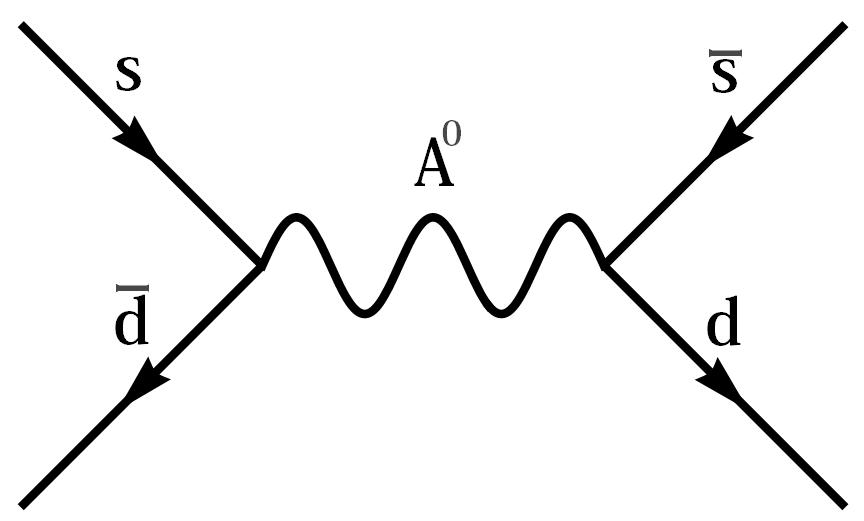
\includegraphics[scale=0.4]{figs/aspon_kaon.png}
\end{center}
\caption{\textit{Feynman Diagram for Kaon mixing in aspon theory }}
\label{asponkaon}
\end{figure}


Generalisations of the aspon model are easy to construct and are the de-facto presentation in \cite{SCPV5}. It is possible to understand what was meant by SCPV being more ``natural" than XCPV in \cite{SCPV1}, simply by thinking that the symmetry breaking mechanism of the Higgs is more natural than the CKM matrix. 


These generalisations simply rely on creating new fields and observing whether or not they have non-removable complex phases in VEVs and their physical effect after symmetry breaking. To be totally general the symmetry breaking need not be Higgs, but for all intents and purposes it usually will be.

In these generalised theories, the particles generated are called ``spurions" of which the $\chi^\alpha$ Higgs particles are specific examples of. SCPV is always related to symmetry breaking of the $\mathrm{U}(1)$ lie group, otherwise, despite VEV having complex phase, it will not show physically. Another important point is the requirement for at least two spurions, for even if there were a non-removable vacuum value like
\begin{align*}
\braket{0|\hat{G}_{CP}|0} = r e^{i\theta}
\end{align*}
As there is only one, this phase will never turn up measurably, one requires a phase difference (just as in QM) for it to be physical.

\subsection{Conclusion}
Despite in general having quite an abstract formulation, SCPV is quite an interesting competitor for explaining CPV. Unfortunately, the mathematical details remain beyond the comprehension of the writer's current abilities. Hence, interesting ideas like exactly how new states are predicted have not been attempted. Still, seeing how complex ideas in particle physical physics can be represented by simple symmetry conditions, just as complex ideas can be represented by Feynman diagrams, makes it a far more approachable subject for an undergraduate.

As what has been discussed is such a general condition it is quite robust to how long it may remain experimentally unfalsifiable. This is not an attractive quality. One condition for falsification would be if XCPV is found to be necessary, as that would contradict the result of part D. What are perhaps more interesting are explicit SCPV theories which make falsifiable predictions. For example the aspon model makes the prediction that for $K^0$ mixing the CP parameters must $Re(\frac{\epsilon'}{\epsilon}) \leq 10^{-5}$ \cite{SCPV7}. Comparing this to the experimental result given in the Neutral Kaon Mixing section, $Re(\frac{\epsilon'}{\epsilon})=0.00166 \pm 0.00023$ it is seen that the aspon method \textit{has} been falsified. 

Quite a few modern theories are difficult if nigh on impossible to falsify. It is refreshing to have dealt with an idea that has been proven wrong. Still, SCPV remains in many other prominent models. Aspon theory is introduced purely as an explanatory example.
 %Commented out to avoid clutter.

\begin{appendix}
\section{Appendix}
Difficult calculations in here.
\end{appendix}
 
\begin{thebibliography}{10}
%Kaon CPV section
\bibitem{FirstCPV}
J. H. Christenson, J. W. Cronin, V. L. Fitch, and R. Turlay (1964) Phys. Review letters, vol. 13, issue 4 - ``Evidence for the $2 \pi$ Decay of the $K^0_2$ Meson'' 
\bibitem{PDGKaons}
J. Beringer et al. (Particle Data Group), Phys. Rev. D86, 010001 (2012) and 2013 partial update for the 2014 edition - ``2013 Review of Particle Physics'' 
\bibitem{Martin+Shaw}
B.R Martin, G. Shaw, Wiley(2008) - ``Particle Physics, Third Edition'' 
\bibitem{Nakada}
Tatsuya Nakada arXiv:hep-ph/9312290v1 15 Dec 1993 - ``Review on CP Violation''
\bibitem{Christenson_apparatus_ref}
http://large.stanford.edu/courses/2008/ph204/coleman1/  
\bibitem{Measurements_Direct_CPV_Kaons_KTev}
KTeV Collaboration, arXiv:hep-ex/0208007v1 6 Aug 2002 - ``Measurements of Direct CP Violation, CPT Symmetry, and Other Parameters in the Neutral Kaon System'' 
\bibitem{HEPP_intro_Perkins}
Donald H. Perkins, Cambridge University Press, 4th edition - ``Introduction to High Energy Physics'' 
\bibitem{DAmbrosio}
Giancarlo D’Ambrosio and Gino Isidori, arXiv:hep-ph/9611284v1 8 Nov 1996 - ``CP violation in Kaon Decays'' 
\bibitem{AsymmetryPic}
Gjesdal, S. et al. Phys.Lett. B52 (1974) 113 Print-74-1358 (CERN) - ``A Measurement of the K(L)-K(s) Mass Difference from the Charge Asymmetry in Semileptonic Kaon Decays'' 
\bibitem{StrangenessPic}
http://www.hep.phy.cam.ac.uk/~thomson/partIIIparticles/handouts/Handout\_12\_2011.pdf

%Deon CPV section
\bibitem{BabarD0mixing}
The BaBar Collaboration http://arxiv.org/abs/hep-ex/0703020v1 1 Apr 2007 - ``Evidence for $D^{0}–\bar{D}^{0}$ Mixing''
\bibitem{BelleD0mixing}
The Belle Collaboration arXiv:hep-ex/0703036v2 1 Apr 2007 - ``Evidence for $D^{0}–\bar{D}^{0}$ Mixing''
\bibitem{Deon_Mixing_Feyn}
http://inspirehep.net/record/1209003/files/mix-rick.png
\bibitem{Babar_D0_Review}
Giulia Casarosa for the BABAR Collaboration - ``Studies of CP Violation and Mixing in the D Mesons decays from BABAR'' - Journal of Physics: Conference Series 335 (2011) 012043   doi:10.1088/1742-6596/335/1/012043
\bibitem{Kevin}
Kevin Maguire, C. Parkes, M. Vesterinen - ``New tagged $D^{0} \rightarrow h h \pi^{0}$ stripping lines'' - LHCb-INT-2013-049 October 1, 2013
\bibitem{Deon_CopOut}
The BaBar Collaboration - ``Improved measurement of the CKM angle $\gamma$ in $B^{\pm} \rightarrow D^{(*)}K^{(*)\mp}$ decays with a Dalitz plot analysis of D decays to $K^{0}_S \pi^{+} \pi^{-}$ and $K^{0}_{S} K^{+} K^{−}$'' - arXiv:0804.2089v2 [hep-ex] 7 Aug 2008
\bibitem{LHCbAsymmetry}
The LHCb Collaboration - ``Measurements of indirect CP asymmetries in $D^{0} \rightarrow K^{+}K^{-}$ and $D^{0} \rightarrow \pi^{+} \pi^{-}$''- arXiv:1310.7201v1 [hep-ex] 27 Oct 2013


%SCPV SECTION
\bibitem{SCPV1}
Fran\c{c}ois Goffinet, CP3 Seminar, Unit\`{e} de Physique Th\`{e}orique et Math\`{e}matique, U.C.L., December 2003
\bibitem{SCPV2} 
Yoav Achiman, ``Spontaneous CP Violation in SUSY," Physics Letters B, March 2007
\bibitem{SCPV3} 
Peter Szekeres, ``A Course in Modern Mathematical Physics," Cambridge University Press, 2004
\bibitem{SCPV4}
John Baez and John Huerta, ``The Algebra of Grand Unified Theories," Bulletin of the American Mathematical Society, vol 47, May 4 2010
\bibitem{SCPV5}
Howard E. Haber and Ze`ev Surujon, ``Group-theoretic Condition for Spontaneous CP Violation," Physical Review D, Volume 86, Issue 7, October 2012
\bibitem{SCPV6}
Bernard de Wit and Eric Laenen, ``Field Theory in Particle Physics" Lecture Notes, Universiteit Utrecht, 2009 http://www.staff.science.uu.nl/~wit00103/ftip/Ch11.pdf
\bibitem{SCPV7}
Paul H. Frampton and Masayasu Harada, ``Kaon Spontaneous CP Violation Reevaluated," Physical Review D, Volume 59, Issue 1, March 1998


\end{thebibliography}

\end{document}
